\chapter{Specific Requirements} \label{requirements}

\section{External interface requirements}

\subsection{User interfaces}

\paragraph{eMSP} The system should be available to the end users in form of a web page and an accessible mobile application (which will be able to receive in-app notifications). In both cases, the user has to be connected to the internet.

\paragraph{CPMS} The system should be available to the end users in form of a web page. The ease of use is not of the outermost importance, and it's not to be preferred over a more complete and condensed view. Priority should be given to offering all functionalities in the quickest possible way and showing relevant information in the clearest way. Users are required to know how to use the system to fully be able to operate all functionalities (this can be done through the design of a user manual).

\subsection{Hardware interfaces}

\paragraph{eMSP} The eMSP doesn't have any particular hardware constraint, but its frontends should be run on any mobile device and computer (in this case only through a browser). Its backend only needs servers able to respond to the user's queries.

\paragraph{CPMS} The only hardware interface needed to access the CPMS is a computer with an installed browser since all functionalities are being offered through a website.

\subsection{Software interfaces}

\paragraph{APIs} The communication between the different systems should happen thanks to the use of standard APIs. All the systems described in this document should be also able to communicate with external systems which expose the same APIs.

\paragraph{eRoaming} There exists an eRoaming service that is accessible thanks to an API that allows eMSPs to query about available CPOs and their location. It also provides the eMSP with the endpoint address of every selected CPMS (CPO's backend).

\paragraph{OpenStreetMap} The eMSP application uses the OpenStreetMap API to provide the map of all the connected charging stations of the various CPOs.

\section{Functional requirements}

\subsection{Requirements}

\paragraph{eMSP requirements}

\begin{center}
    \begin{tabular}{ | >{\centering\arraybackslash}m{0.1\columnwidth} | >{\arraybackslash}m{0.84\columnwidth} | }
        \hline
        \textbf{Identifier} & \multicolumn{1}{c|}{\textbf{Description}} \\
        \hline
        \hline
        \showR{r:e:signup} & The system must allow the user to sign-up. \\
        \hline
        \showR{r:e:signup_check} & The system must check the sign-up data. \\
        \hline
    \end{tabular}
\end{center}
\begin{center}
    \begin{tabular}{ | >{\centering\arraybackslash}m{0.1\columnwidth} | >{\arraybackslash}m{0.84\columnwidth} | }
        \hline
        \textbf{Identifier} & \multicolumn{1}{c|}{\textbf{Description}} \\
        \hline
        \hline
        \showR{r:e:signup_mail} & The system must send the user an email for activating the account after a successful sign-up. \\
        \hline
        \showR{r:e:signup_activation} & The system must discard any account activation request that arrives after 24 hours from the sign-up procedure. \\
        \hline
        \showR{r:e:signup_not_activated} & The system must consider any signed-up user who hasn't already activated the account as an unregistered user. \\
        \hline
        \showR{r:e:signup_success} & The system must notify the user of the sign-up result, sending an email if it's successful. \\
        \hline
        \showR{r:e:login} & The system must allow the user to log in. \\
        \hline
        \showR{r:e:login_check} & The system must check the login data. \\
        \hline
        \showR{r:e:pwchange} & The system must allow the user to change his/her password after logging in. \\
        \hline
        \showR{r:e:pwreset} & The system must allow any registered user to reset his/her password by sending an email to the specified address. \\
        \hline
        \showR{r:e:pwreset_timeout} & The system must discard any password change 24 hours after the request. \\
        \hline
        \showR{r:e:pwreset_duplicate} & The system must discard any duplicated usage of the same link for password change after a successful one. \\
        \hline
        \showR{r:e:logout} & The system must allow the user to logout. \\
        \hline
        \showR{r:e:notification} & The system must allow the user to set the preferred notification method. \\
        \hline
        \showR{r:e:car_add} & The system must allow the user to add a new vehicle. \\
        \hline
        \showR{r:e:car_remove} & The system must allow the user to remove an associated vehicle, only if there is at least one. \\
        \hline
        \showR{r:e:car_edit} & The system must allow the user to edit any associated vehicle's details. \\
        \hline
        \showR{r:e:stations_lookup} & The system must allow the user to look for nearby stations. \\
        \hline
        \showR{r:e:stations_sort} & The system must allow the user to sort the nearby stations according to distance, price, and availability. \\
        \hline
        \showR{r:e:stations_favorite_mark} & The system must allow the user to mark and unmark stations as \doublequotes{favorite}. \\
        \hline
        \showR{r:e:book} & The system must allow the user to book a charge in a charging station if any slot is available. \\
        \hline
        \showR{r:e:book_car} & The system must ask the user the vehicle s/he wants to charge every time s/he books a charge. \\
        \hline
        \showR{r:e:book_notification} & The system must notify the user of any successful booked charge. \\
        \hline
        \showR{r:e:book_add_calendar} & The system must allow the user to add any booked charge to the calendar. \\
        \hline
        \showR{r:e:book_all} & The system must allow the user to show all the booked charges, both past, and future (there might be limits). \\
        \hline
        \showR{r:e:book_edit} & The system must allow the user to edit or delete a booked charge before the end of the booked slot. \\
        \hline
        \showR{r:e:book_notification_slot} & The system must notify the user of the charging slot to use before the charge. \\
        \hline
        \showR{r:e:book_notification_end} & The system must notify the user when the charge is finished. \\
        \hline
        \showR{r:e:payment} & The system must allow the user to pay for the obtained service. \\
        \hline
        \showR{r:e:payment_notification} & The system must notify the user after every payment attempt (both in case of success and failure). \\
        \hline
        \showR{r:e:eroaming} & The system must periodically contact an eRoaming service for obtaining the list of available CPOs (and respective CPMSs). \\
        \hline
        \showR{r:e:cpms_connect} & The system must be able to connect to any CPMS that offers standard APIs. \\
        \hline
        \showR{r:e:cpms_communicate} & The system must be able to communicate with any connected CPMS through standard APIs. \\
        \hline
        \showR{r:e:user_registered} & The system must allow any registered user to do everything specified, except signing up. \\
        \hline
        \showR{r:e:user_unregistered} & The system must allow any unregistered user to only sign up and log in. \\
        \hline
        \showR{r:e:notification_app} & The system must send the notification only to the user's authenticated devices if the notification preference is by in-app notification. \\
        \hline
        \showR{r:e:notification_mail} & The system must send emails instead of in-app notifications if that's the user's preferred method or if there is no available user's device. \\
        \hline
    \end{tabular}
\end{center}

\pagebreak

\paragraph{CPMS requirements}

\begin{center}
    \begin{tabular}{ | >{\centering\arraybackslash}m{0.1\columnwidth} | >{\arraybackslash}m{0.84\columnwidth} | }
        \hline
        \textbf{Identifier} & \multicolumn{1}{c|}{\textbf{Description}} \\
        \hline
        \hline
        \showR{r:c:input} & The system must check all input data correctness. \\
        \hline
        \showR{r:c:login} & The system must allow the user to log in. \\
        \hline
        \showR{r:c:pwchange} & The system must allow the user to change his/her password after logging in. \\
        \hline
        \showR{r:c:pwreset} & The system must allow any registered user to reset his/her password by sending an email to the specified address. \\
        \hline
        \showR{r:c:pwreset_timeout} & The system must discard any password change 24 hours after the request. \\
        \hline
        \showR{r:c:pwreset_duplicate} & The system must discard any duplicated usage of the same link for password change after a successful one. \\
        \hline
        \showR{r:c:logout} & The system must allow the user to logout. \\
        \hline
        \showR{r:c:API_show_booking} & The system must provide an API function to get information about all bookings present for any charging station. \\
        \hline
        \showR{r:c:API_book} & The system must provide an API function to add/delete a booking for a charging point in a charging station. \\
        \hline
        \showR{r:c:API_stations} & The system must provide an API function to get information about all charging points and respective sockets in a charging station. \\
        \hline
        \showR{r:c:API_prices} & The system must provide an API function to get information about prices relative to a charging station and socket types. \\
        \hline
        \showR{r:c:start_car_charge} & The system must start charging a car when it is first plugged in if it corresponds to the car for which a charge was booked in the corresponding time and place (same charging point/socket as well). \\
        \hline
        \showR{r:c:stop_car_charge_full} & The system must stop charging a car once it recognizes that the car battery has reached full capacity. \\
        \hline
        \showR{r:c:stop_car_charge_time} & The system must stop charging a car if the booking corresponding to that car ends and the car is still plugged in. \\
        \hline
        \showR{r:c:autoselect_DSO} & The system must automatically select the DSO that offers the best energy price if the “automatic DSO choice” is selected. \\
        \hline
        \showR{r:c:stop_battery_charge_full} & If a battery was charging and reaches a full charge, the system must stop charging the battery. \\
        \hline
        \showR{r:c:auto_mix} & The system must automatically change the energy mix if the \doublequotes{automatic mix choice} is selected. \\
        \hline
        \showR{r:c:notification_column} & The system must automatically notify the eMSP of the assignment of a charging column. \\
        \hline
        \showR{r:c:notification_charge} & The system must automatically notify the eMSP of the end of the car charge. \\
        \hline
        \showR{r:c:periodical_updates} & The system must periodically update the database with new data coming from sensors present in charging stations. \\
        \hline
        \showR{r:c:view_bookings} & The system must allow the CPMS user to view all bookings present for any charging station. \\
        \hline
        \showR{r:c:view_charging_point} & The system must allow the CPMS user to view all charging points, relative socket types, and if they are occupied or not, for any charging station. \\
        \hline
        \showR{r:c:view_battery_levels} & The system must allow the CPMS user to view the batteries' charge levels if present. \\
        \hline
        \showR{r:c:manage_offers} & The system must allow the CPMS user to create and delete special charge offers. \\
        \hline
        \showR{r:c:view_DSO} & The system must allow the CPMS user to view all DSO available. \\
        \hline
        \showR{r:c:view_DSO_prices} & The system must allow the CPMS user to view all DSO prices. \\
        \hline
        \showR{r:c:change_mix} & The system must allow the CPMS user to change the energy mix. \\
        \hline
        \showR{r:c:start_battery_charge} & The system must allow the CPMS user to start recharging batteries if they are present. \\
        \hline
        \showR{r:c:auto_DSO} & The system must allow the CPMS user to activate and deactivate \doublequotes{automatic DSO choice}. \\
        \hline
        \showR{r:c:auto_MIX} & The system must allow the CPMS user to activate and deactivate \doublequotes{automatic mix choice}. \\
        \hline
        \showR{r:c:DSO_payment} & The system must allow the CPMS user to modify the automatic DSO payment method. \\
    \hline
    \end{tabular}
\end{center}

\pagebreak

\subsection{Goal mapping}

\paragraph{eMSP goals}

\begin{center}
    \begin{tabular}{ | >{\centering\arraybackslash\bfseries}m{0.06\columnwidth} | >{\arraybackslash}m{0.36\columnwidth} | >{\arraybackslash}m{0.5\columnwidth} | }
        \hline
        Goal & \multicolumn{1}{c|}{\textbf{Domain assumptions}} & \multicolumn{1}{c|}{\textbf{Requirements}} \\
        \hline
        \hline
        \refG{g:e:lookup} & \refD{d:connect}, \refD{d:truth}, \refD{d:reliable}, \refD{d:api}, \refD{d:eroaming} & \refR{r:e:signup}-\refR{r:e:notification}, \refR{r:e:stations_lookup}, \refR{r:e:stations_sort}, \refR{r:e:stations_favorite_mark}, \refR{r:e:eroaming}, \refR{r:e:cpms_connect}, \refR{r:e:cpms_communicate}, \refR{r:e:user_registered}, \refR{r:e:user_unregistered} \\
        \hline
        \refG{g:e:book} & \refD{d:connect}, \refD{d:truth}, \refD{d:vehicle}, \refD{d:reliable}, \refD{d:api} & \refR{r:e:signup}-\refR{r:e:notification}, \refR{r:e:car_add}-\refR{r:e:car_edit}, \refR{r:e:book}-\refR{r:e:book_notification_slot}, \refR{r:e:cpms_communicate}, \refR{r:e:user_registered}-\refR{r:e:notification_mail} \\
        \hline
        \refG{g:e:start} & \refD{d:plug}-\refD{d:vehicle}, \refD{d:abusive}-\refD{d:unauthorized}, \refD{d:dso_energy}, \refD{d:socket}, \refD{d:reliable}, \refD{d:api} & \refR{r:e:car_add}-\refR{r:e:car_edit}, \refR{r:e:cpms_communicate}, \refR{r:e:user_registered}, \refR{r:e:user_unregistered} \\
        \hline
        \refG{g:e:notify} & \refD{d:connect}, \refD{d:truth}, \refD{d:charge}, \refD{d:reliable}, \refD{d:api} & \refR{r:e:signup}-\refR{r:e:notification}, \refR{r:e:car_add}-\refR{r:e:car_edit}, \refR{r:e:book_notification_end}, \refR{r:e:cpms_communicate}, \refR{r:e:user_registered}-\refR{r:e:notification_mail}, \refR{r:c:notification_column}, \refR{r:c:notification_charge} \\
        \hline
        \refG{g:e:pay} & \refD{d:connect}, \refD{d:truth}, \refD{d:harm}, \refD{d:charge}-\refD{d:api} & \refR{r:e:signup}-\refR{r:e:notification}, \refR{r:e:car_add}-\refR{r:e:car_edit}, \refR{r:e:payment}, \refR{r:e:payment_notification}, \refR{r:e:user_registered}-\refR{r:e:notification_mail} \\
        \hline
    \end{tabular}
\end{center}

\paragraph{CPMS goals}

\begin{center}
    \begin{tabular}{ | >{\centering\arraybackslash\bfseries}m{0.06\columnwidth} | >{\arraybackslash}m{0.36\columnwidth} | >{\arraybackslash}m{0.5\columnwidth} | }
        \hline
        Goal & \multicolumn{1}{c|}{\textbf{Domain assumptions}} & \multicolumn{1}{c|}{\textbf{Requirements}} \\
        \hline
        \hline
        \refG{g:c:info} & \refD{d:vehicle}, \refD{d:abusive}, \refD{d:harm}, \refD{d:batteries}, \refD{d:charge}, \refD{d:reliable} & \refR{r:e:book}, \refR{r:e:book_all}, \refR{r:e:book_edit}, \refR{r:e:book_notification_slot}, \refR{r:c:API_show_booking}-\refR{r:c:API_prices}, \refR{r:c:periodical_updates}, \refR{r:c:view_bookings}-\refR{r:c:view_battery_levels} \\
        \hline
        \refG{g:c:charge} & \refD{d:vehicle}, \refD{d:abusive}-\refD{d:unauthorized}, \refD{d:dso_energy}-\refD{d:reliable}, \refD{d:api}, \refD{d:cpo} & \refR{r:c:API_show_booking}, \refR{r:c:start_car_charge}-\refR{r:c:stop_car_charge_time}, \refR{r:c:notification_column}, \refR{r:c:notification_charge} \\
        \hline
        \refG{g:c:dso} & \refD{d:connect}, \refD{d:dso}, \refD{d:reliable}, \refD{d:api}, \refD{d:cpo} & \refR{r:c:input}-\refR{r:c:logout}, \refR{r:c:autoselect_DSO}, \refR{r:c:view_DSO}, \refR{r:c:view_DSO_prices}, \refR{r:c:auto_DSO}, \refR{r:c:DSO_payment} \\
        \hline
        \refG{g:c:mix} & \refD{d:connect}, \refD{d:dso}, \refD{d:batteries}, \refD{d:dso_energy}, \refD{d:reliable}, \refD{d:api}, \refD{d:cpo} & \refR{r:c:input}-\refR{r:c:logout}, \refR{r:c:stop_battery_charge_full}, \refR{r:c:auto_mix}, \refR{r:c:change_mix}, \refR{r:c:start_battery_charge}, \refR{r:c:auto_MIX} \\
        \hline
        \refG{g:c:offers} & \refD{d:connect}, \refD{d:reliable}, \refD{d:api}, \refD{d:cpo} & \refR{r:c:input}-\refR{r:c:logout}, \refR{r:c:API_prices}, \refR{r:c:manage_offers}, \refR{r:c:view_DSO_prices} \\
        \hline
    \end{tabular}
\end{center}

\subsection{Users' use cases diagrams}

\begin{figure}[h!]
    \centering
    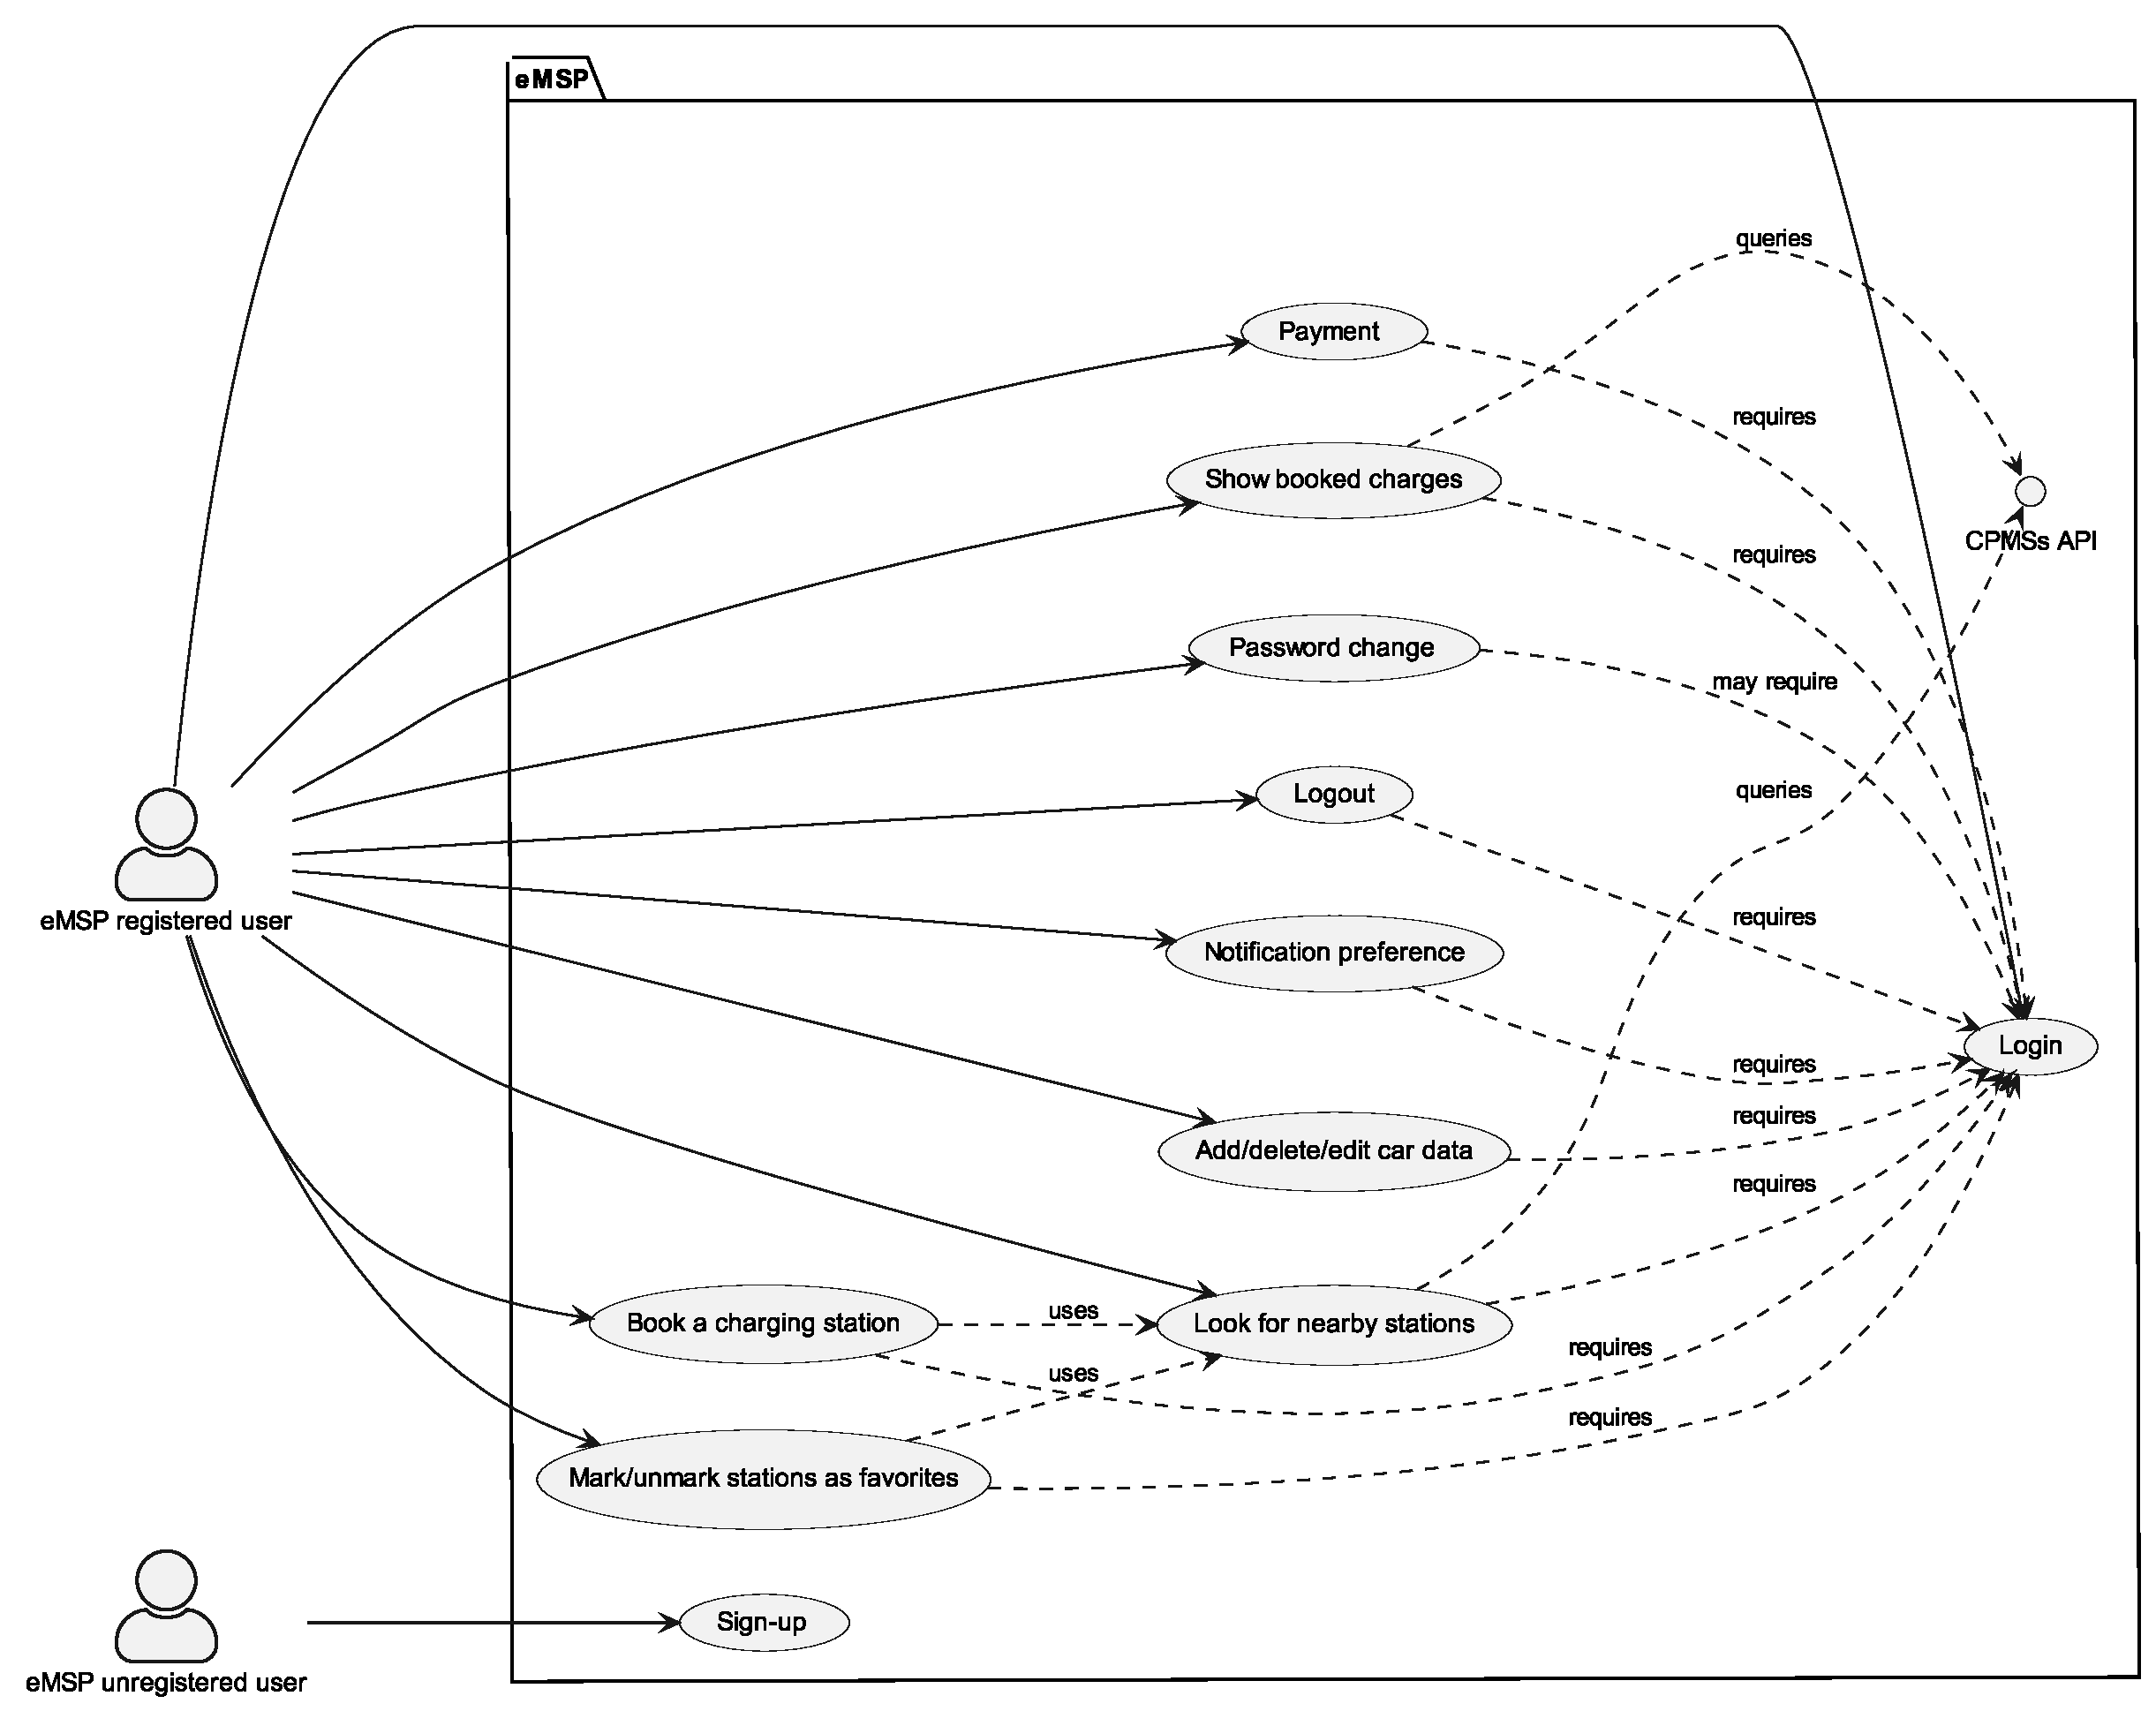
\includegraphics[width=\columnwidth]{./images/diagrams/usecases/emsp}
    \caption{eMSP users' use cases.}
\end{figure}

\begin{figure}[h!]
    \centering
    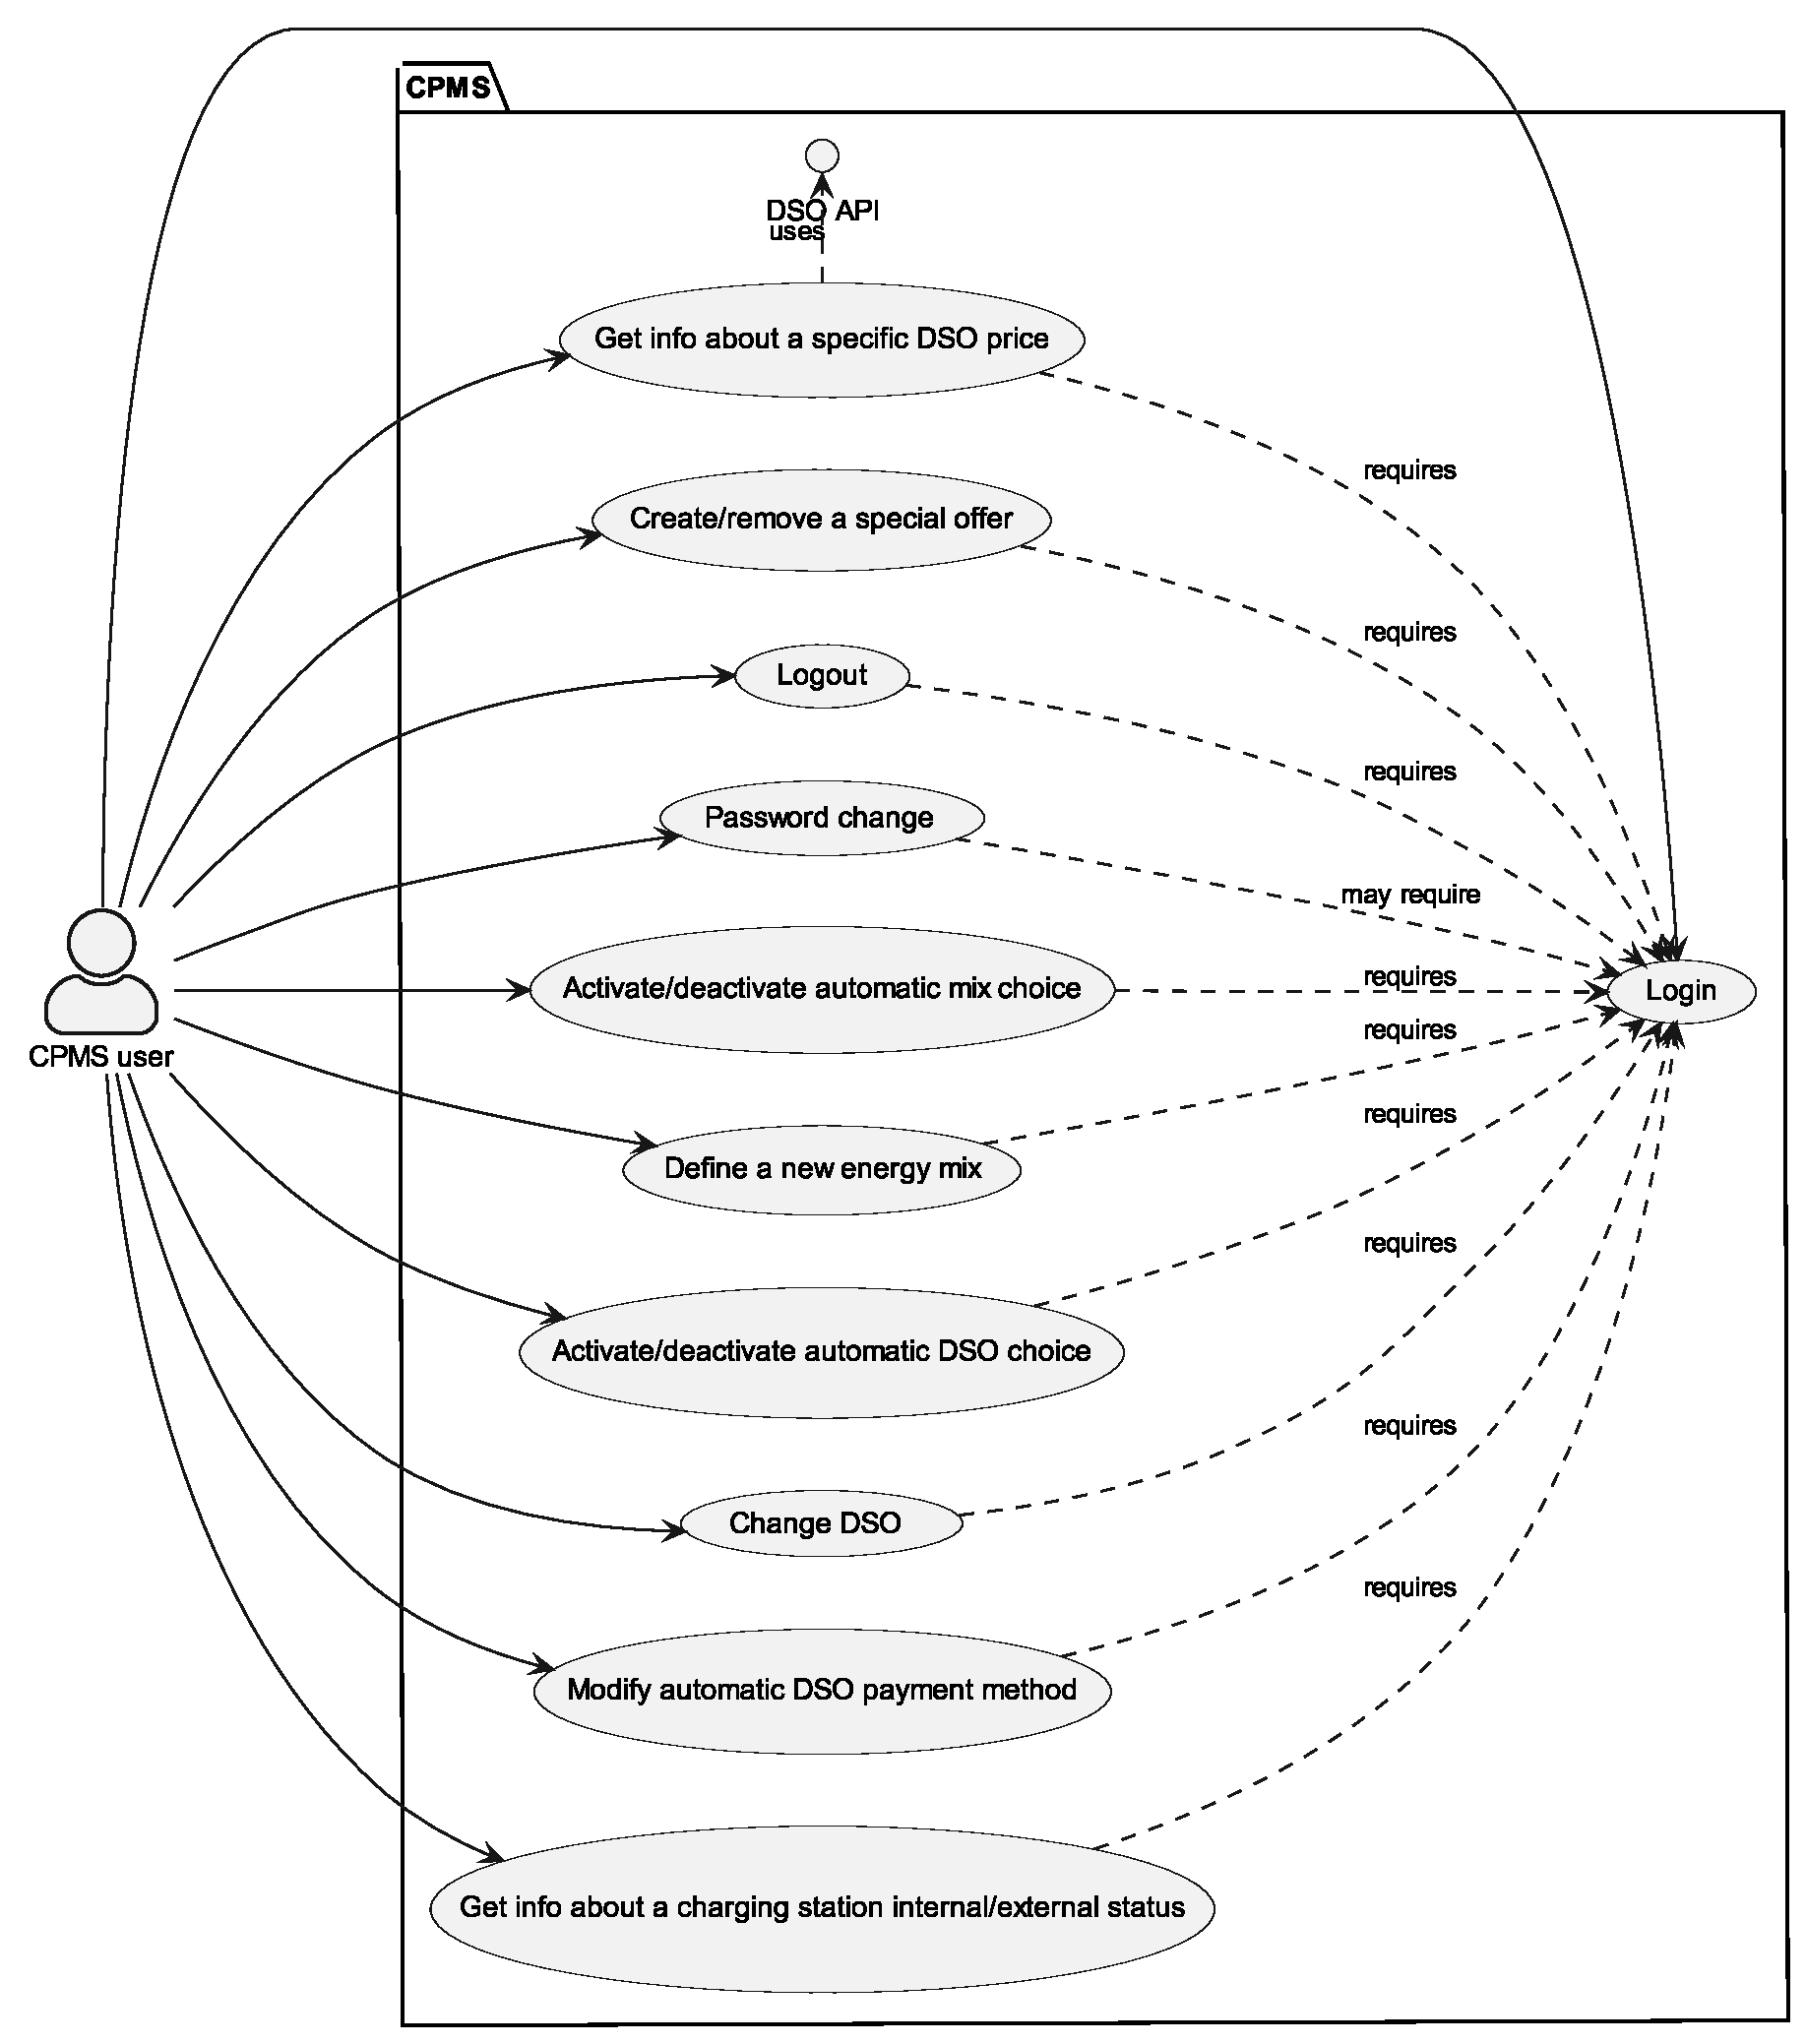
\includegraphics[width=0.8\columnwidth]{./images/diagrams/usecases/cpms}
    \caption{CPMS users' use cases.}
\end{figure}

\subsection{Use cases}

Every time \doublequotes{consumer} or \doublequotes{user} appears in a UML diagram, it's intended that s/he is interacting with the application or web page that interacts with the system.\medskip

For the sake of simplicity, many data checks and the opening of the application or web page, according to the use case, are not illustrated, but they are present in the system. Moreover, some cases are not depicted here:
\begin{itemize}
    \item \textit{Notification preference}: the user is asked to choose between in-app notifications or email ones after his first login. Furthermore, the user can change this preference at any time under his/her profile.
    \item \textit{Logout}: simply removes the token\footnote{An explanation of the usage of the token can be found in the eMSP's login use case (\refUC{uc:e:login}).} from the client.
    \item \textit{Password change}: it works like most of the password changes implemented nowadays. The first option is that the user clicks on the \doublequotes{Forgot password?} link, receives an email with the link for changing it, and changes the password. The second one is that s/he goes to the user's details page and changes the password directly from there. In both cases, s/he has to log back in on all his/her connected devices.
\end{itemize}
Also, even if it's not specified in the diagrams, if any component fails, the user is notified and the action is automatically aborted, reverting its state to the original one. The same happens in case of user's network failures (which are \doublequotes{detected}\footnote{This is a simplification, since in a distributed environment with possible byzantine failures things are a bit more complex.} through a timeout).

\vfill
\pagebreak

\paragraph{eMSP | Registration}

\begin{center}
    \begin{tabular}{ | >{\arraybackslash}m{0.17\columnwidth} | >{\arraybackslash}m{0.77\columnwidth} | }
        \hline
        \textbf{Identifier} & \showUC{uc:e:registration} \\
        \hline
        \textbf{Actor} & Consumer (end user) \\
        \hline
        \textbf{Entry condition} & The user is not already registered \\
        \hline
        \textbf{Event flow} & \medskip\parbox[b][][b]{0.76\columnwidth}{
            \begin{enumerate}[nosep, leftmargin=*]
                \item The user opens the application or webpage
                \item The user fills out the registration form
                \item The system checks the inserted data
                \item The system sends an email to the user for confirming the account
                \item The user clicks on the link for activating the account
                \item The system notifies that the account is confirmed
            \end{enumerate}
        } \\
        \hline
        \textbf{Exit condition} & The process ends without errors \\
        \hline
        \textbf{Exceptions} & \medskip\parbox[b][][b]{0.76\columnwidth}{
            \begin{itemize}[nosep, leftmargin=*]
                \item There is already a registered user with that email address
                \item The passwords don't coincide
                \item The user doesn't click on the link in the email within 24 hours
            \end{itemize}
        } \\
        \hline
        \textbf{Special requests} & The user needs to have access to an email address \\
        \hline
    \end{tabular}
\end{center}

\begin{figure}[h!]
    \centering
    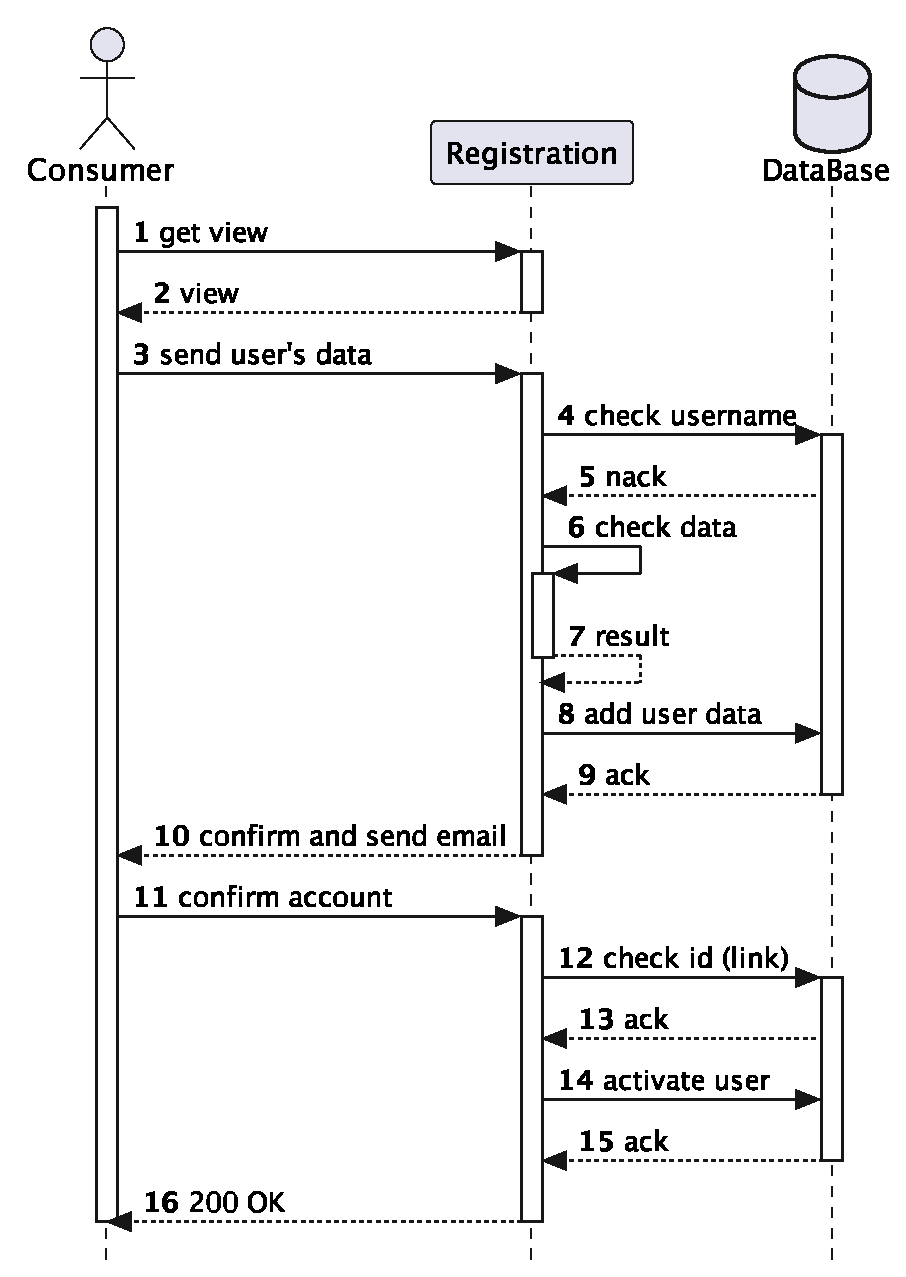
\includegraphics[width=0.46\columnwidth]{./images/diagrams/sequences/emsp/registration}
    \caption{registration of the eMSP user (consumer).}
\end{figure}

\pagebreak

\paragraph{eMSP | Login}

\begin{center}
    \begin{tabular}{ | >{\arraybackslash}m{0.17\columnwidth} | >{\arraybackslash}m{0.77\columnwidth} | }
        \hline
        \textbf{Identifier} & \showUC{uc:e:login} \\
        \hline
        \textbf{Actor} & Consumer (end user) \\
        \hline
        \textbf{Entry condition} & The user is already registered \\
        \hline
        \textbf{Event flow} & \medskip\parbox[b][][b]{0.76\columnwidth}{
            \begin{enumerate}[nosep, leftmargin=*]
                \item The user opens the application or webpage
                \item The user fills out the login form
                \item The system checks the inserted data
                \item The system logs in the user sending back a token with all the information
            \end{enumerate}
        } \\
        \hline
        \textbf{Exit condition} & The process ends without errors and the token is sent \\
        \hline
        \textbf{Exceptions} & \medskip\parbox[b][][b]{0.76\columnwidth}{
            \begin{itemize}[nosep, leftmargin=*]
                \item The inserted username corresponds to a non-activated account
                \item The username doesn't exist
                \item The password hash doesn't coincide
            \end{itemize}
        } \\
        \hline
    \end{tabular}
\end{center}

\begin{figure}[h!]
    \centering
    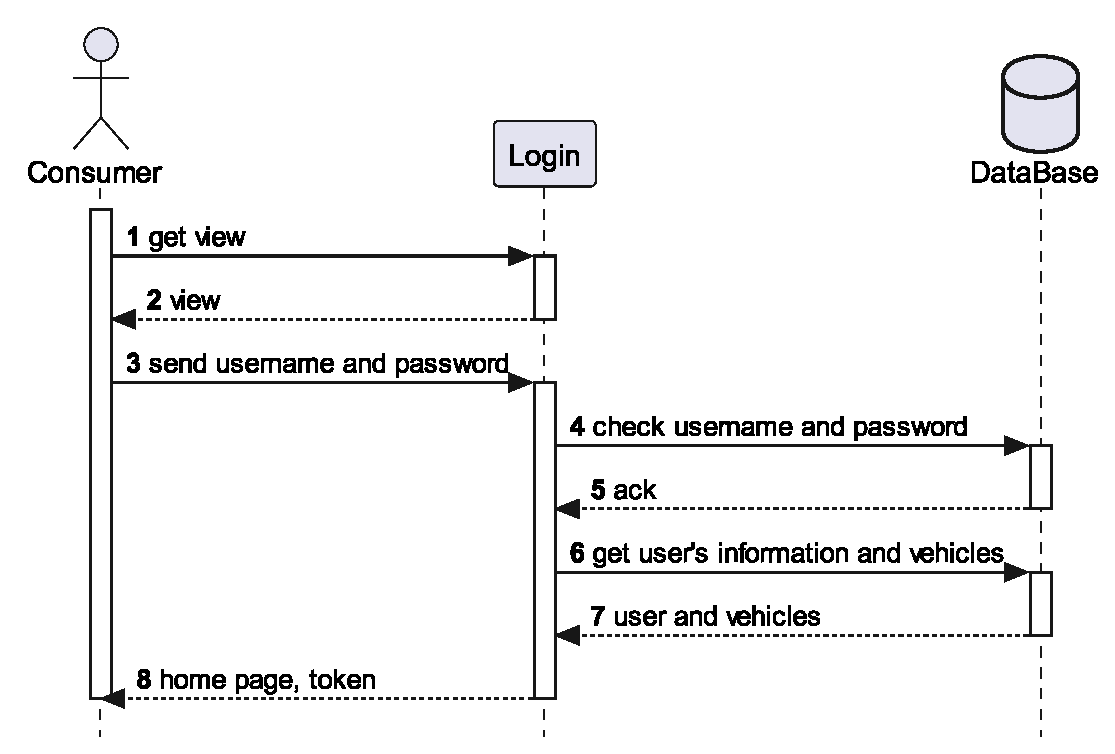
\includegraphics[width=0.62\columnwidth]{./images/diagrams/sequences/emsp/login}
    \caption{login of the eMSP user (consumer).}
\end{figure}

Please, note that the token present in the scheme is to be intended like a JWT with all the information of the user (which can fit into the token because of their small size) that has to be sent every time. This explains why certain pieces of information are not queried every time they are needed.

\pagebreak

\paragraph{eMSP | Vehicles editing}

\begin{center}
    \begin{tabular}{ | >{\arraybackslash}m{0.17\columnwidth} | >{\arraybackslash}m{0.77\columnwidth} | }
        \hline
        \textbf{Identifier} & \showUC{uc:e:vehicles} \\
        \hline
        \textbf{Actor} & Consumer (end user) \\
        \hline
        \textbf{Entry condition} & The user needs to add/remove/edit one or more associated vehicles \\
        \hline
        \textbf{Event flow} & \medskip\parbox[b][][b]{0.76\columnwidth}{
            \begin{enumerate}[nosep, leftmargin=*]
                \item The user opens the list of vehicles
                \item The user adds a new vehicle (inserting all the data) or clicks on one
                \item If the user clicks on a vehicle, he can choose to edit or remove it
                \item The system confirms the operation, sends back an updated token, and updates any future reservation (deleting it if the vehicle is deleted or editing it with the new certificate)
            \end{enumerate}
        } \\
        \hline
        \textbf{Exit condition} & The process ends without errors \\
        \hline
        \textbf{Exceptions} & \medskip\parbox[b][][b]{0.76\columnwidth}{
            \begin{itemize}[nosep, leftmargin=*]
                \item The user tries to remove some information from a vehicle while editing
            \end{itemize}
        } \\
        \hline
        \textbf{Special requests} & If the user wants to add a new vehicle or to change the certificate of any, s/he has to be able to upload the certificate \\
        \hline
    \end{tabular}
\end{center}

\begin{figure}[h!]
    \centering
    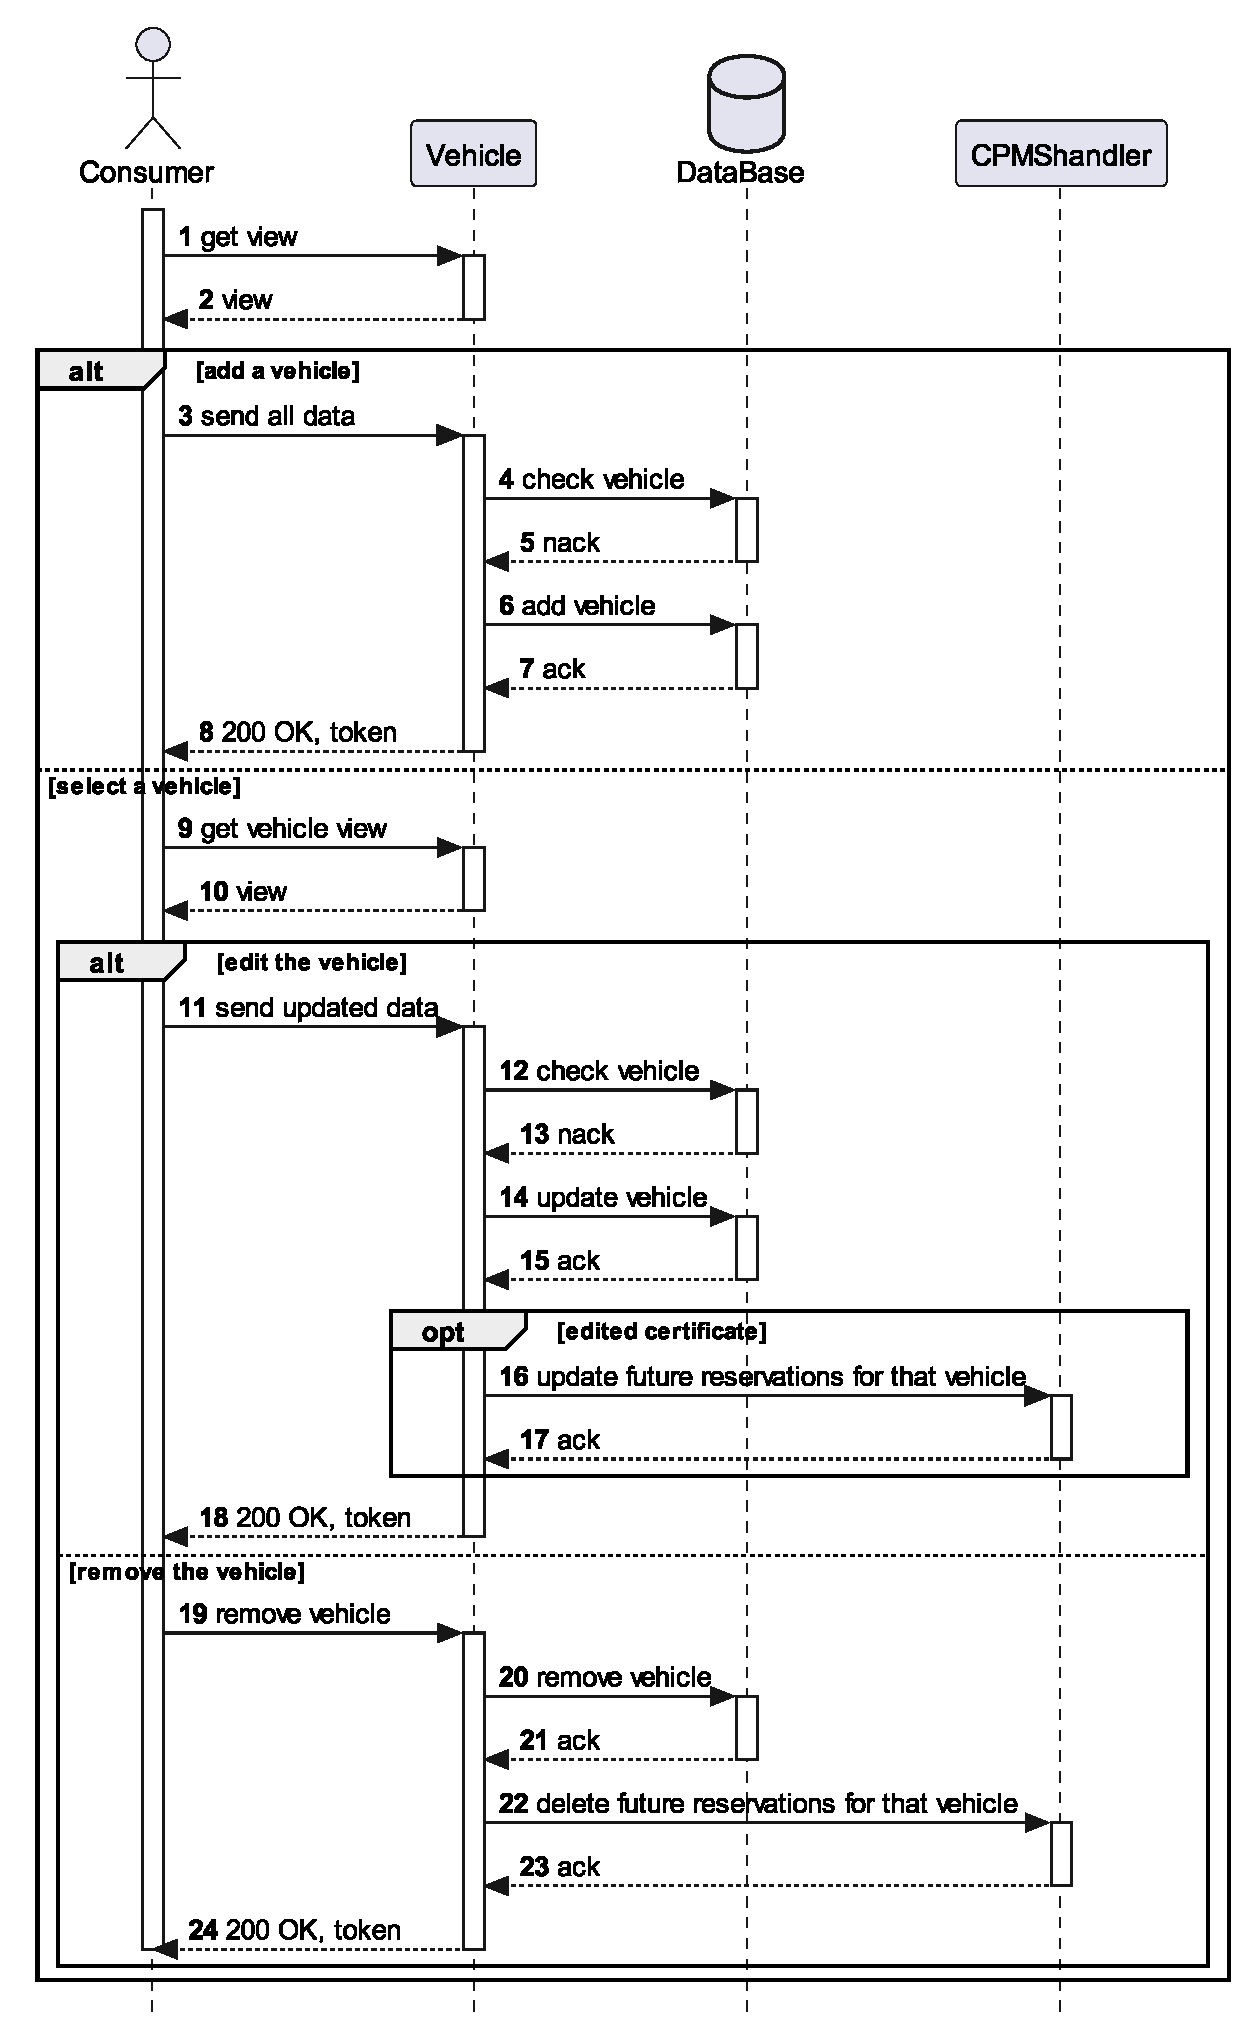
\includegraphics[width=0.59\columnwidth]{./images/diagrams/sequences/emsp/vehicles}
    \caption{the user manages his/her vehicles.}
\end{figure}

\pagebreak

\paragraph{eMSP | Look for nearby stations}

\begin{center}
    \begin{tabular}{ | >{\arraybackslash}m{0.17\columnwidth} | >{\arraybackslash}m{0.77\columnwidth} | }
        \hline
        \textbf{Identifier} & \showUC{uc:e:stations_lookup} \\
        \hline
        \textbf{Actor} & Consumer (end user) \\
        \hline
        \textbf{Entry condition} & The user is already logged in \\
        \hline
        \textbf{Event flow} & \medskip\parbox[b][][b]{0.76\columnwidth}{
            \begin{enumerate}[nosep, leftmargin=*]
                \item The user opens the map page (if s/he selects the favorites, skips to the last point)
                \item The user activates the geolocalization or searches for a place
                \item If wanted, the user clicks on the list view (s/he can switch at any time)
                \item If the user is in the list view, s/he can sort the stations based on some parameters
                \item The user opens the details of the charging station, eventually toggling favorite
            \end{enumerate}
        } \\
        \hline
        \textbf{Exit condition} & The process ends without errors \\
        \hline
        \textbf{Exceptions} & \medskip\parbox[b][][b]{0.76\columnwidth}{
            \begin{itemize}[nosep, leftmargin=*]
                \item The user inserts a nonexistent location
            \end{itemize}
        } \\
        \hline
    \end{tabular}
\end{center}

\begin{figure}[h!]
    \centering
    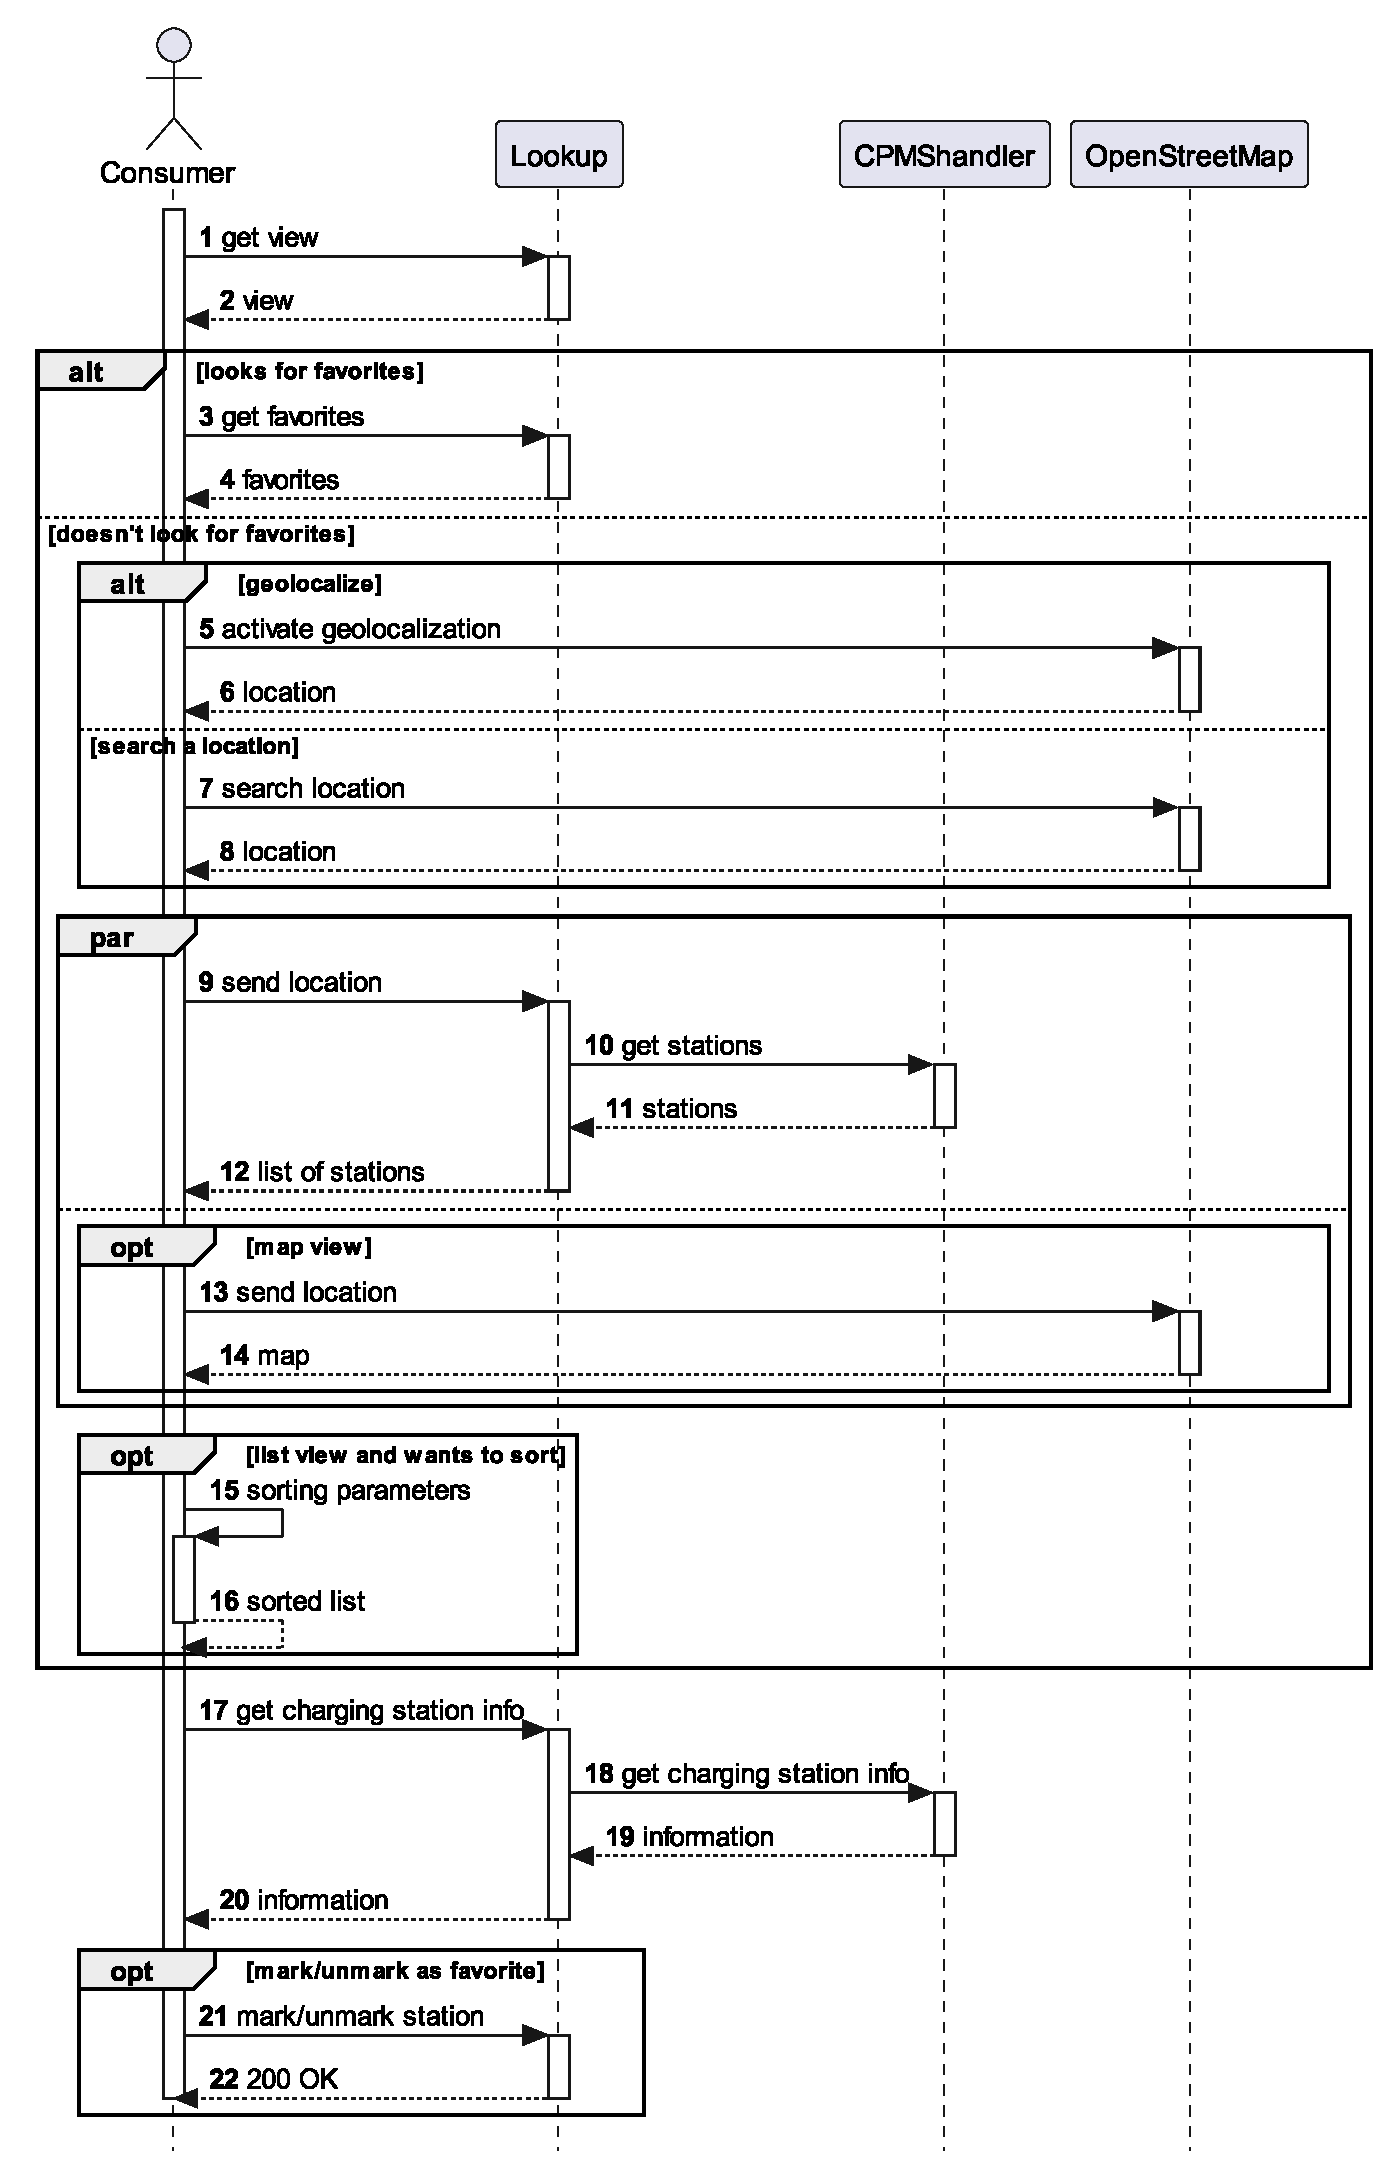
\includegraphics[width=0.67\columnwidth]{./images/diagrams/sequences/emsp/lookup}
    \caption{the user looks for a charging station and marks/unmarks it as \doublequotes{favorite}.}
\end{figure}

\pagebreak

\paragraph{eMSP | Book a charge}

\begin{center}
    \begin{tabular}{ | >{\arraybackslash}m{0.17\columnwidth} | >{\arraybackslash}m{0.77\columnwidth} | }
        \hline
        \textbf{Identifier} & \showUC{uc:e:book} \\
        \hline
        \textbf{Actor} & Consumer (end user) \\
        \hline
        \textbf{Entry condition} & The user has already opened the information of a charging station \\
        \hline
        \textbf{Event flow} & \medskip\parbox[b][][b]{0.76\columnwidth}{
            \begin{enumerate}[nosep, leftmargin=*]
                \item The user opens the book functionality
                \item The user selects the vehicle to charge (only if more than one)
                \item The user selects some available slots
                \item The system notifies the user of the successful operation and sends all the details
            \end{enumerate}
        } \\
        \hline
        \textbf{Exit condition} & The process ends without errors \\
        \hline
        \textbf{Exceptions} & \medskip\parbox[b][][b]{0.76\columnwidth}{
            \begin{itemize}[nosep, leftmargin=*]
                \item The user has no associated vehicle
                \item There are no available slots for that charging station and socket
                \item The user selects a duration that exceeds the maximum duration for that slot
                \item Some other user, meanwhile, has booked even a small part of the selected slot
            \end{itemize}
        } \\
        \hline
    \end{tabular}
\end{center}

\begin{figure}[h!]
    \centering
    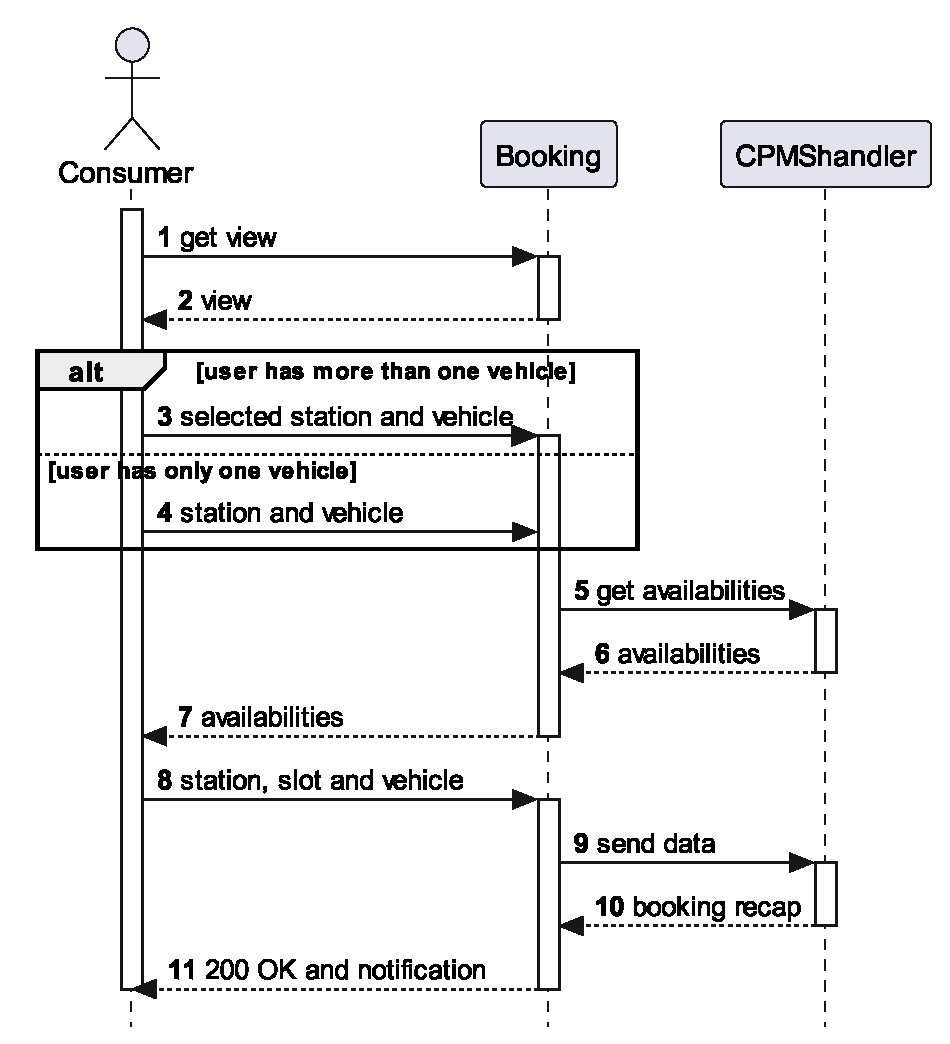
\includegraphics[width=0.5\columnwidth]{./images/diagrams/sequences/emsp/book}
    \caption{the user books a charge.}
\end{figure}

\pagebreak

\paragraph{eMSP | Edit/delete a reservation}

\begin{center}
    \begin{tabular}{ | >{\arraybackslash}m{0.17\columnwidth} | >{\arraybackslash}m{0.77\columnwidth} | }
        \hline
        \textbf{Identifier} & \showUC{uc:e:edit} \\
        \hline
        \textbf{Actor} & Consumer (end user) \\
        \hline
        \textbf{Entry condition} & The user has already booked a charge and needs to edit or delete it \\
        \hline
        \textbf{Event flow} & \medskip\parbox[b][][b]{0.76\columnwidth}{
            \begin{enumerate}[nosep, leftmargin=*]
                \item The user accesses the list of future charges
                \item The user selects a charge
                \item The user edits (following steps 2-4 of \refUC{uc:e:book}) or deletes it
                \item The system notifies the change
            \end{enumerate}
        } \\
        \hline
        \textbf{Exit condition} & The process ends without errors \\
        \hline
        \textbf{Exceptions} & \medskip\parbox[b][][b]{0.76\columnwidth}{
            \begin{itemize}[nosep, leftmargin=*]
                \item The user tries to delete a past or current charge
                \item An exception from the booking process ones (\refUC{uc:e:book}) arises
            \end{itemize}
        } \\
        \hline
    \end{tabular}
\end{center}

\begin{figure}[h!]
    \centering
    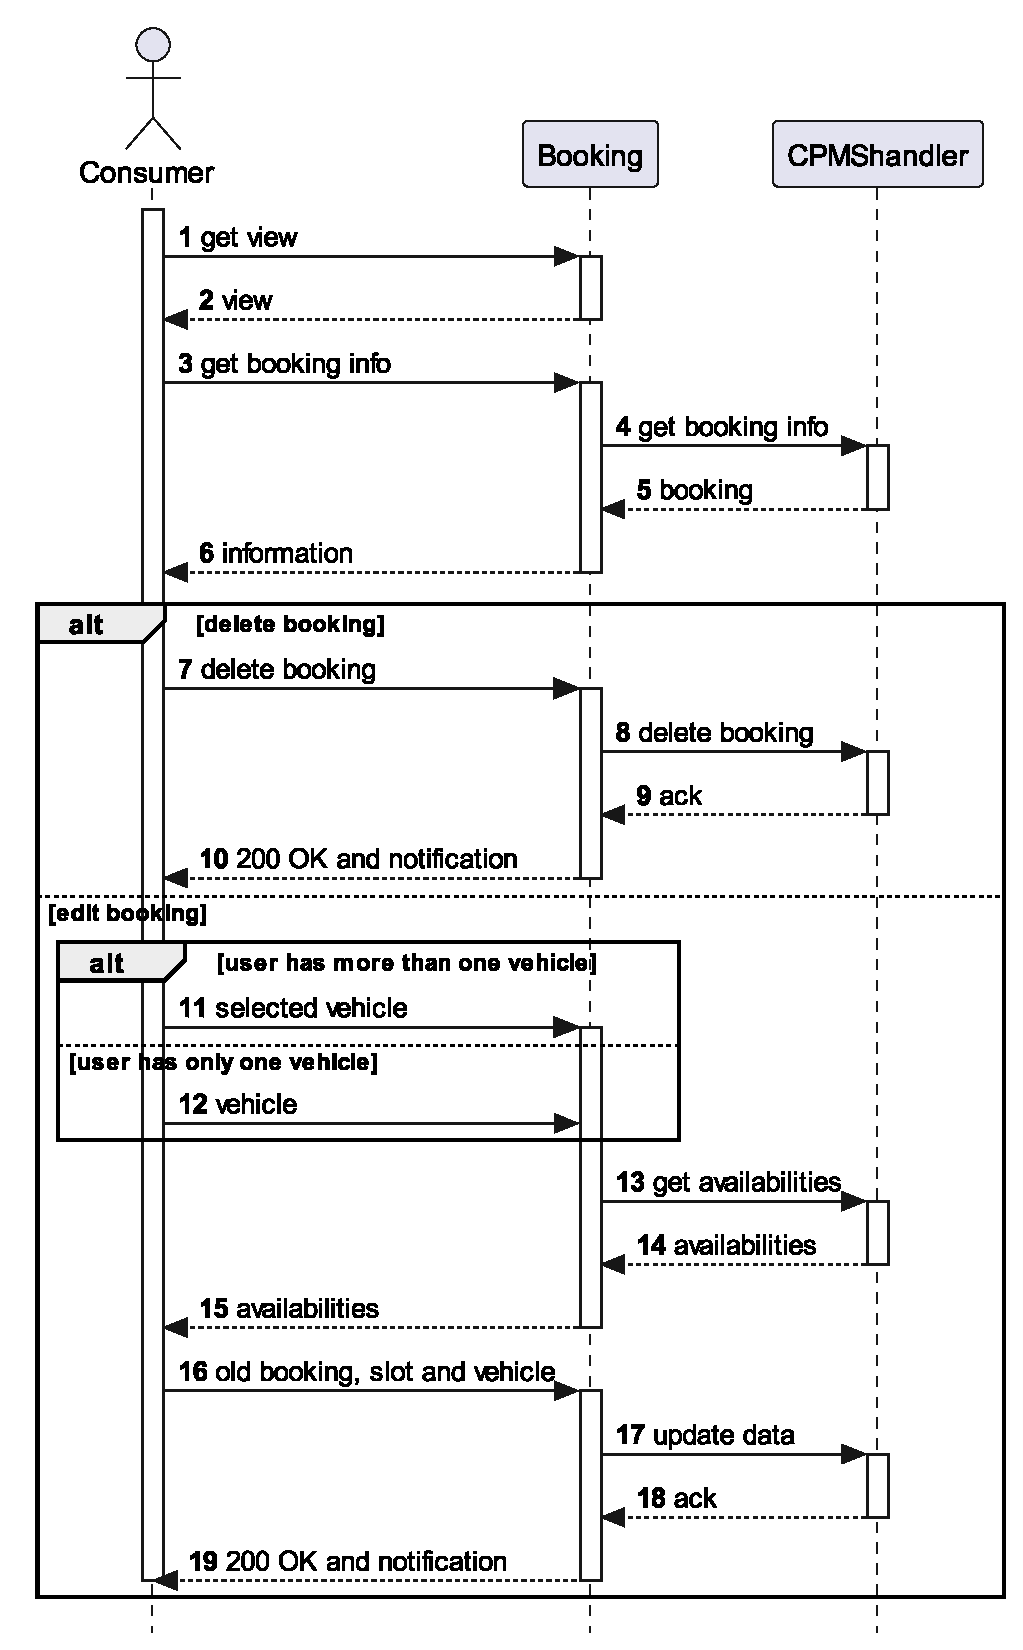
\includegraphics[width=0.57\columnwidth]{./images/diagrams/sequences/emsp/edit}
    \caption{the user edits or removes a booked charge.}
\end{figure}

\pagebreak

\paragraph{eMSP | Get notified}

\begin{center}
    \begin{tabular}{ | >{\arraybackslash}m{0.17\columnwidth} | >{\arraybackslash}m{0.77\columnwidth} | }
        \hline
        \textbf{Identifier} & \showUC{uc:e:notification} \\
        \hline
        \textbf{Actor} & Consumer (end user) \\
        \hline
        \textbf{Entry condition} & The system is informed about an important fact for the user (assigned socket, end of charge, or payment result) \\
        \hline
        \textbf{Event flow} & \medskip\parbox[b][][b]{0.76\columnwidth}{
            \begin{enumerate}[nosep, leftmargin=*]
                \item The system checks the user's notification preferences
                \item The system notifies the user
            \end{enumerate}
        } \\
        \hline
        \textbf{Exit condition} & The notification is sent to the user \\
        \hline
    \end{tabular}
\end{center}

\begin{figure}[h!]
    \centering
    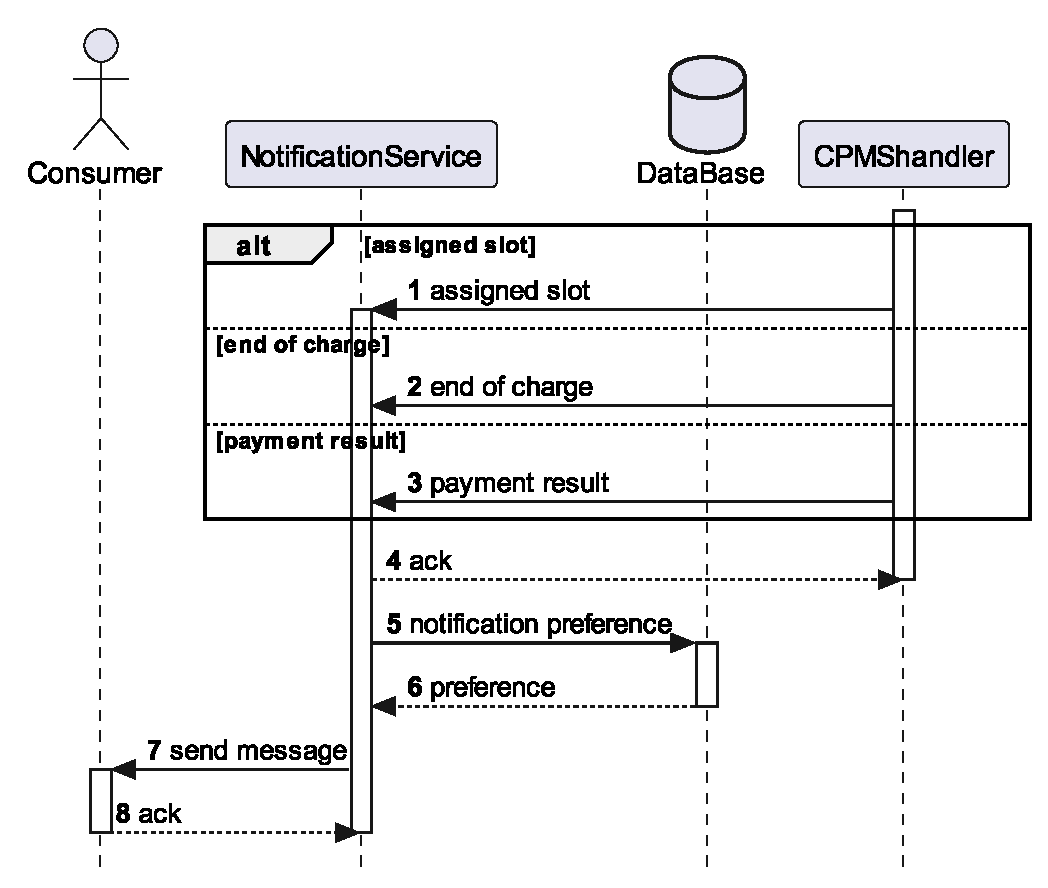
\includegraphics[width=0.55\columnwidth]{./images/diagrams/sequences/emsp/notification}
    \caption{the system notifies the user about an important fact from the CPMS.}
\end{figure}

Since these three cases are close to each other, they are represented together in the same use case.

\pagebreak

\paragraph{eMSP | Pay for the obtained service}

\begin{center}
    \begin{tabular}{ | >{\arraybackslash}m{0.17\columnwidth} | >{\arraybackslash}m{0.77\columnwidth} | }
        \hline
        \textbf{Identifier} & \showUC{uc:e:payment} \\
        \hline
        \textbf{Actor} & Consumer (end user) \\
        \hline
        \textbf{Entry condition} & After completing a charge, the user has to pay for it \\
        \hline
        \textbf{Event flow} & \medskip\parbox[b][][b]{0.76\columnwidth}{
            \begin{enumerate}[nosep, leftmargin=*]
                \item The user selects the charge to pay
                \item The system redirects the user to the payment page
                \item The user inserts the data
                \item The system confirms the payment and notifies the CPMS and the user
            \end{enumerate}
        } \\
        \hline
        \textbf{Exit condition} & The process ends without errors \\
        \hline
        \textbf{Exceptions} & \medskip\parbox[b][][b]{0.76\columnwidth}{
            \begin{itemize}[nosep, leftmargin=*]
                \item The user inserts wrong payment data
            \end{itemize}
        } \\
        \hline
        \textbf{Special requests} & The user has a valid payment method \\
        \hline
    \end{tabular}
\end{center}

\begin{figure}[h!]
    \centering
    
\includegraphics[width=0.66\columnwidth]{./images/diagrams/sequences/emsp/payment}
    \caption{the user pays for the charge.}
\end{figure}

Similar to this, the in-loco payment requires the user to insert his/her payment data (or to use a payment card, according to how it's implemented) and in this case it's the CPMS who notifies the eMSP, and not the other way round.

\pagebreak

\paragraph{CPMS | Login}

\begin{center}
    \begin{tabular}{ | >{\arraybackslash}m{0.17\columnwidth} | >{\arraybackslash}m{0.77\columnwidth} | }
        \hline
        \textbf{Identifier} & \showUC{uc:c:login} \\
        \hline
        \textbf{Actor} & CPO allowed user \\
        \hline
        \textbf{Entry condition} &  The user is at the login page in the website\\
        \hline
        \textbf{Event flow} & \medskip\parbox[b][][b]{0.76\columnwidth}{
            \begin{enumerate}[nosep, leftmargin=*]
                \item The user enters login data
                \item The system checks if input data matches database content
                \item The system queries the DBMS for home page data
                \item The system sends back the home page with all relevant information 
            \end{enumerate}
        } \\
        \hline
        \textbf{Exit condition} & The process ends without errors \\
        \hline
        \textbf{Exceptions} & \medskip\parbox[b][][b]{0.76\columnwidth}{
            \begin{itemize}[nosep, leftmargin=*]
                \item Missing or wrong input data is sent from the user
            \end{itemize}
        } \\
        \hline
    \end{tabular}
\end{center}

\begin{figure}[h!]
    \centering
    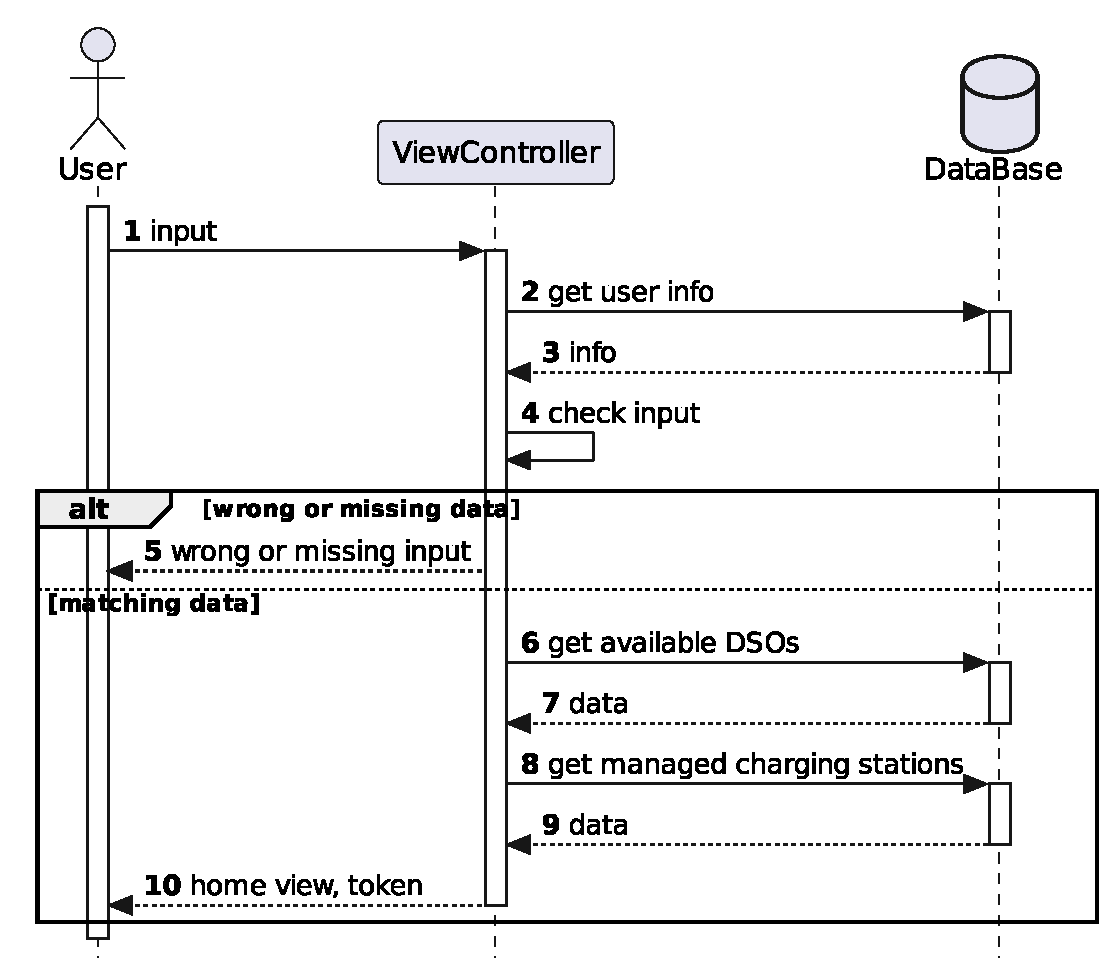
\includegraphics[width=0.65\columnwidth]{./images/diagrams/sequences/cpms/login}
    \caption{login of a registered CPO user.}
\end{figure}

\pagebreak

\paragraph{CPMS | Check charging station status}


\begin{center}
    \begin{tabular}{ | >{\arraybackslash}m{0.17\columnwidth} | >{\arraybackslash}m{0.77\columnwidth} | }
        \hline
        \textbf{Identifier} & \showUC{uc:c:infStation} \\
        \hline
        \textbf{Actor} & CPO allowed user \\
        \hline
        \textbf{Entry condition} &  The user is at the home page in the website\\
        \hline
        \textbf{Event flow} & \medskip\parbox[b][][b]{0.76\columnwidth}{
            \begin{enumerate}[nosep, leftmargin=*]
                \item The user selects a charging station
                \item The user selects \doublequotes{Check status}
                \item The system queries the DBMS for all relevant information
                \item The DBMS returns all relevant information
                \item The system sends back the new page with all relevant information 
                \item The system periodically sends new information to the website
            \end{enumerate}
        } \\
        \hline
        \textbf{Exit condition} & The process ends without errors \\
        \hline
        \textbf{Exceptions} & \medskip\parbox[b][][b]{0.76\columnwidth}{
            \begin{itemize}[nosep, leftmargin=*]
                \item A non-existing charging station is selected
                \item The selected charging station is not managed by the user
            \end{itemize}
        } \\
        \hline
    \end{tabular}
\end{center}

\begin{figure}[h!]
    \centering
    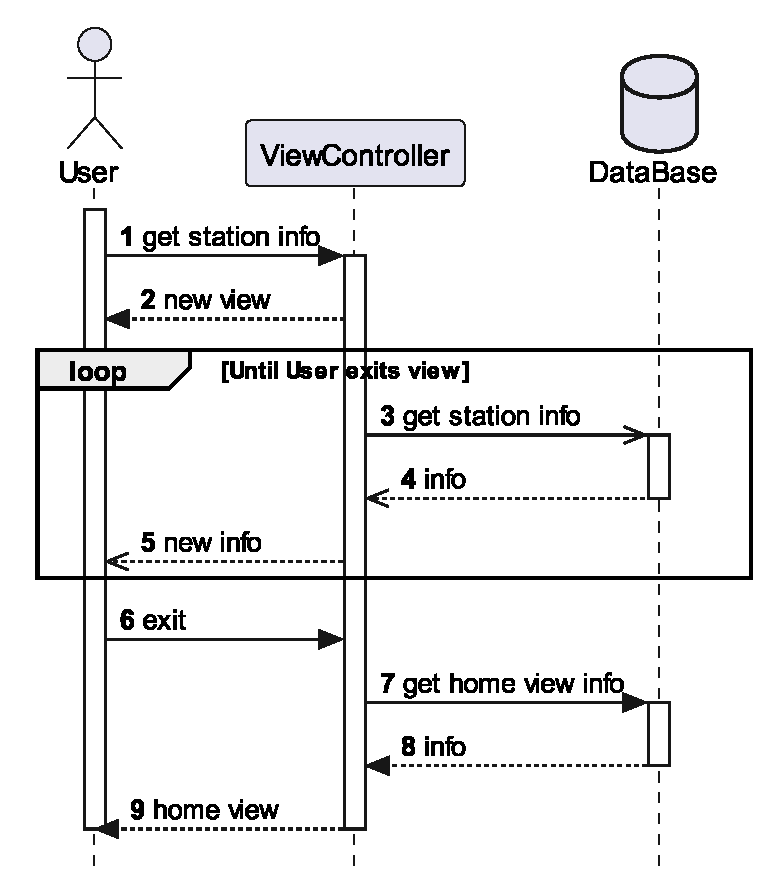
\includegraphics[width=0.50\columnwidth]{./images/diagrams/sequences/cpms/infStation}
    \caption{change view from the home page to charging station info.}
\end{figure}

As stated in requirement \refR{r:c:periodical_updates}, the system periodically has to update the database with information regarding all changing parameters coming from charging stations. These include the station's battery levels, incoming energy from the solar panels, occupied columns in the station, and eventually more data. This allows the view controller to simply fetch data from the database, instead of intercepting all data streams, to communicate to the website in the corresponding views.

\pagebreak

\paragraph{CPMS | Change energy mix}

\begin{center}
    \begin{tabular}{ | >{\arraybackslash}m{0.17\columnwidth} | >{\arraybackslash}m{0.77\columnwidth} | }
        \hline
        \textbf{Identifier} & \showUC{uc:c:changeMix} \\
        \hline
        \textbf{Actor} & CPO allowed user \\
        \hline
        \textbf{Entry condition} & The user is at the home page in the website \\
        \hline
        \textbf{Event flow} & \medskip\parbox[b][][b]{0.76\columnwidth}{
            \begin{enumerate}[nosep, leftmargin=*]
                \item The user selects \doublequotes{Change energy mix}
                \item The user defines a new energy mix
                \item The system communicates the new energy mix to the charging station
                \item The charging station communicates the components the change
            \end{enumerate}
        } \\
        \hline
        \textbf{Exit condition} & A new energy mix is defined without errors, the user is notified \\
        \hline
        \textbf{Exceptions} & \medskip\parbox[b][][b]{0.76\columnwidth}{
            \begin{itemize}[nosep, leftmargin=*]
                \item The new energy mix could not be attained 
                \item The database could not be updated 
                \item The user could not be notified 
            \end{itemize}
        } \\
        \hline
        \textbf{Special requests} & The user has to input a reasonable energy mix \\
        \hline
    \end{tabular}
\end{center}

\begin{figure}[h!]
    \centering
    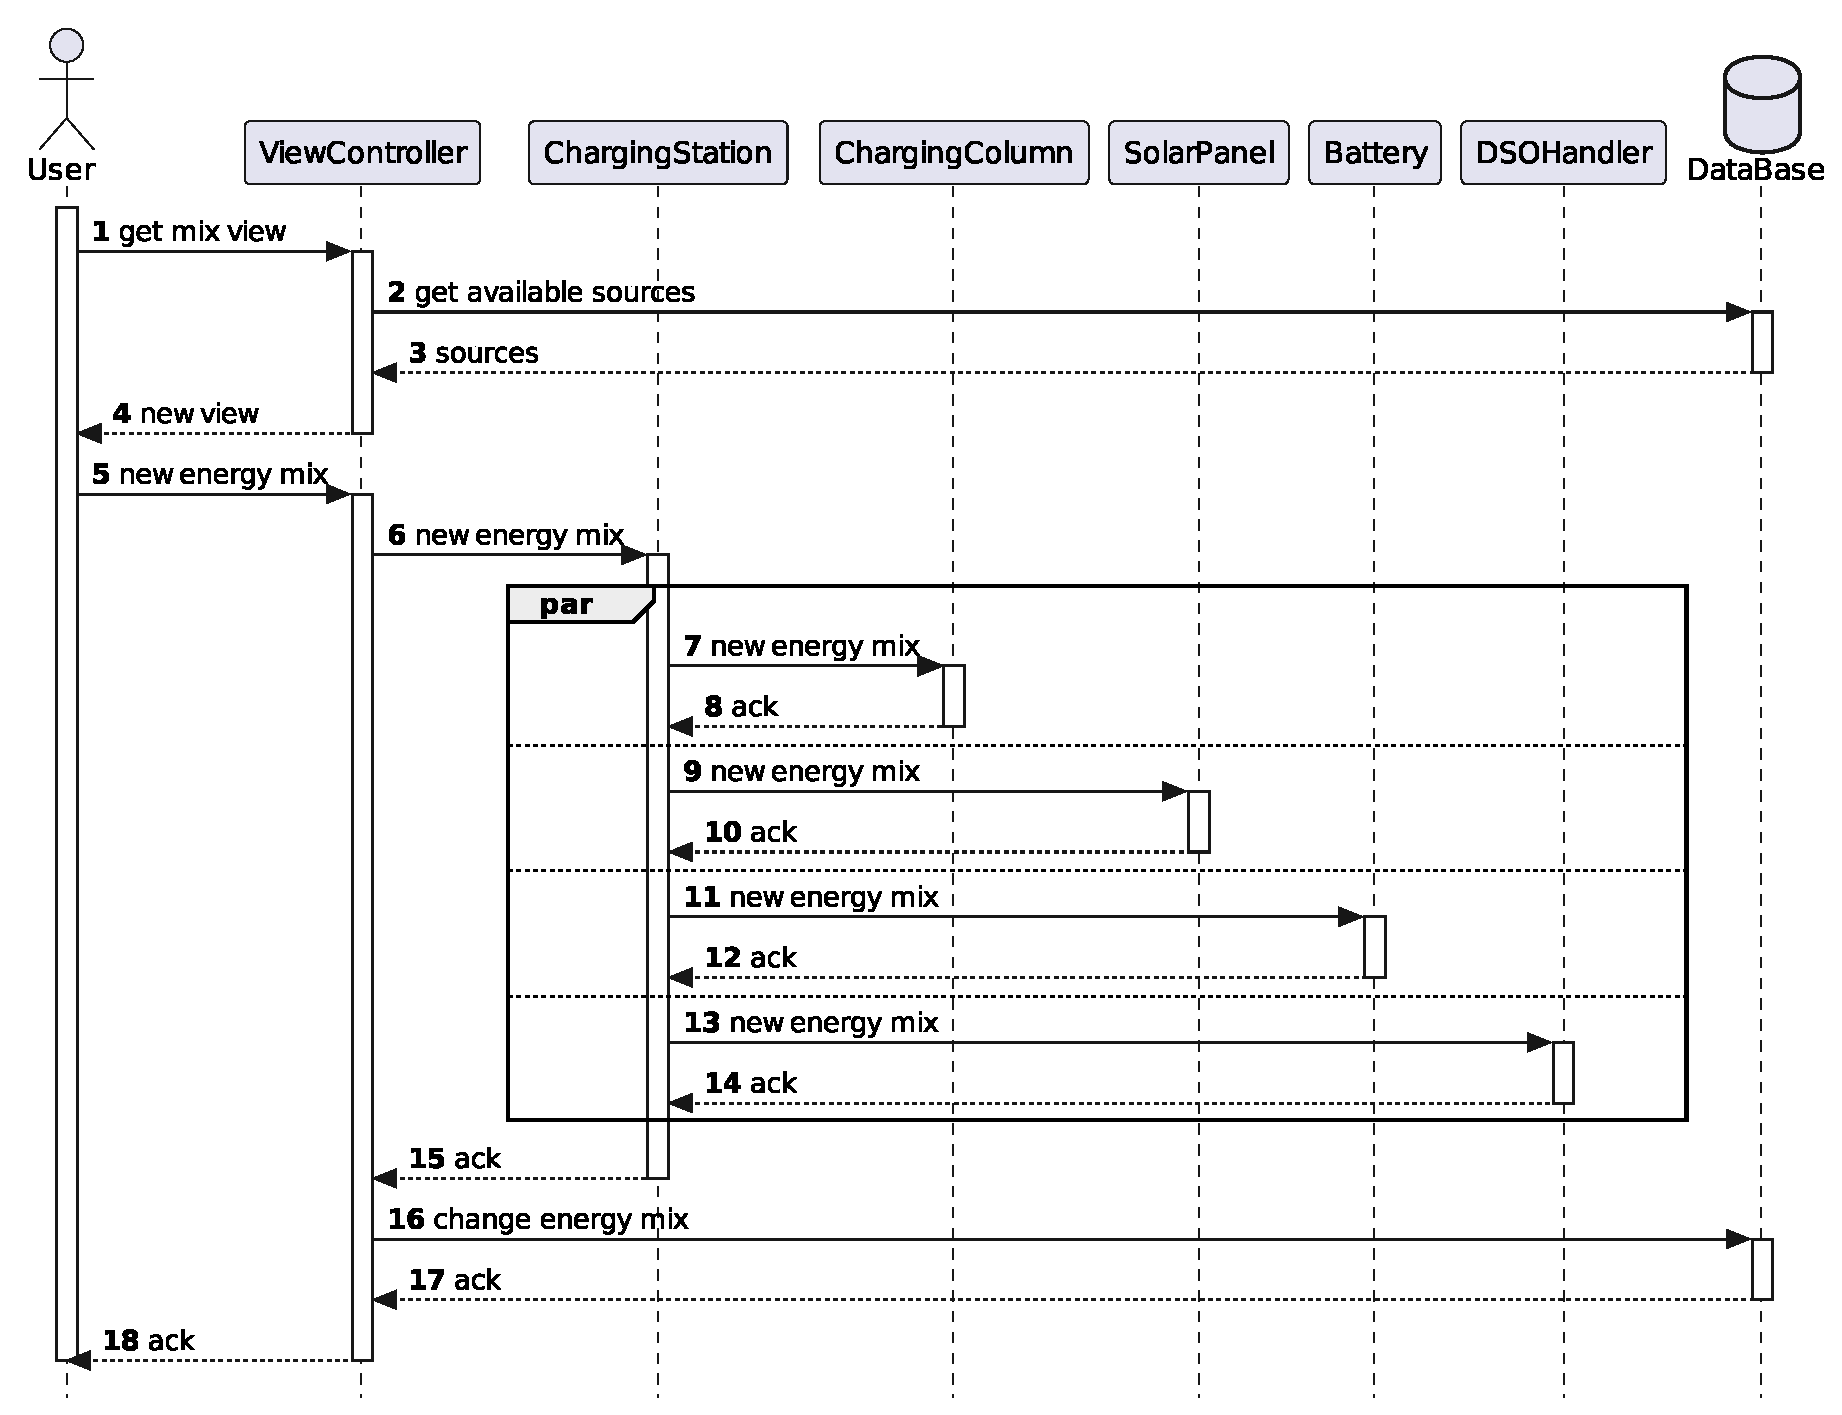
\includegraphics[width=1\columnwidth]{./images/diagrams/sequences/cpms/energyMix}
    \caption{user changing energy mix of a charging station.}
\end{figure}

\pagebreak

\paragraph{CPMS | Manage DSO choice}

\begin{center}
    \begin{tabular}{ | >{\arraybackslash}m{0.17\columnwidth} | >{\arraybackslash}m{0.77\columnwidth} | }
        \hline
        \textbf{Identifier} & \showUC{uc:c:DSO} \\
        \hline
        \textbf{Actor} & CPO allowed user \\
        \hline
        \textbf{Entry condition} & The user is at the home page in the website \\
        \hline
        \textbf{Event flow} & \medskip\parbox[b][][b]{0.76\columnwidth}{
            \begin{enumerate}[nosep, leftmargin=*]
                \item The user selects a charging station
                \item The user selects \doublequotes{Available DSO}
                \item The system sends a new DSO view
                \item The user selects a DSO
                \item The system starts using the selected DSO in the charging station
            \end{enumerate}
        } \\
        \hline
        \textbf{Exit condition} & The DSO is being used in the charging station and the user is notified \\
        \hline
        \textbf{Exceptions} & \medskip\parbox[b][][b]{0.76\columnwidth}{
            \begin{itemize}[nosep, leftmargin=*]
                \item The DSO stops being available while the choice is being made
            \end{itemize}
        } \\
        \hline
    \end{tabular}
\end{center}

\begin{figure}[h!]
    \centering
    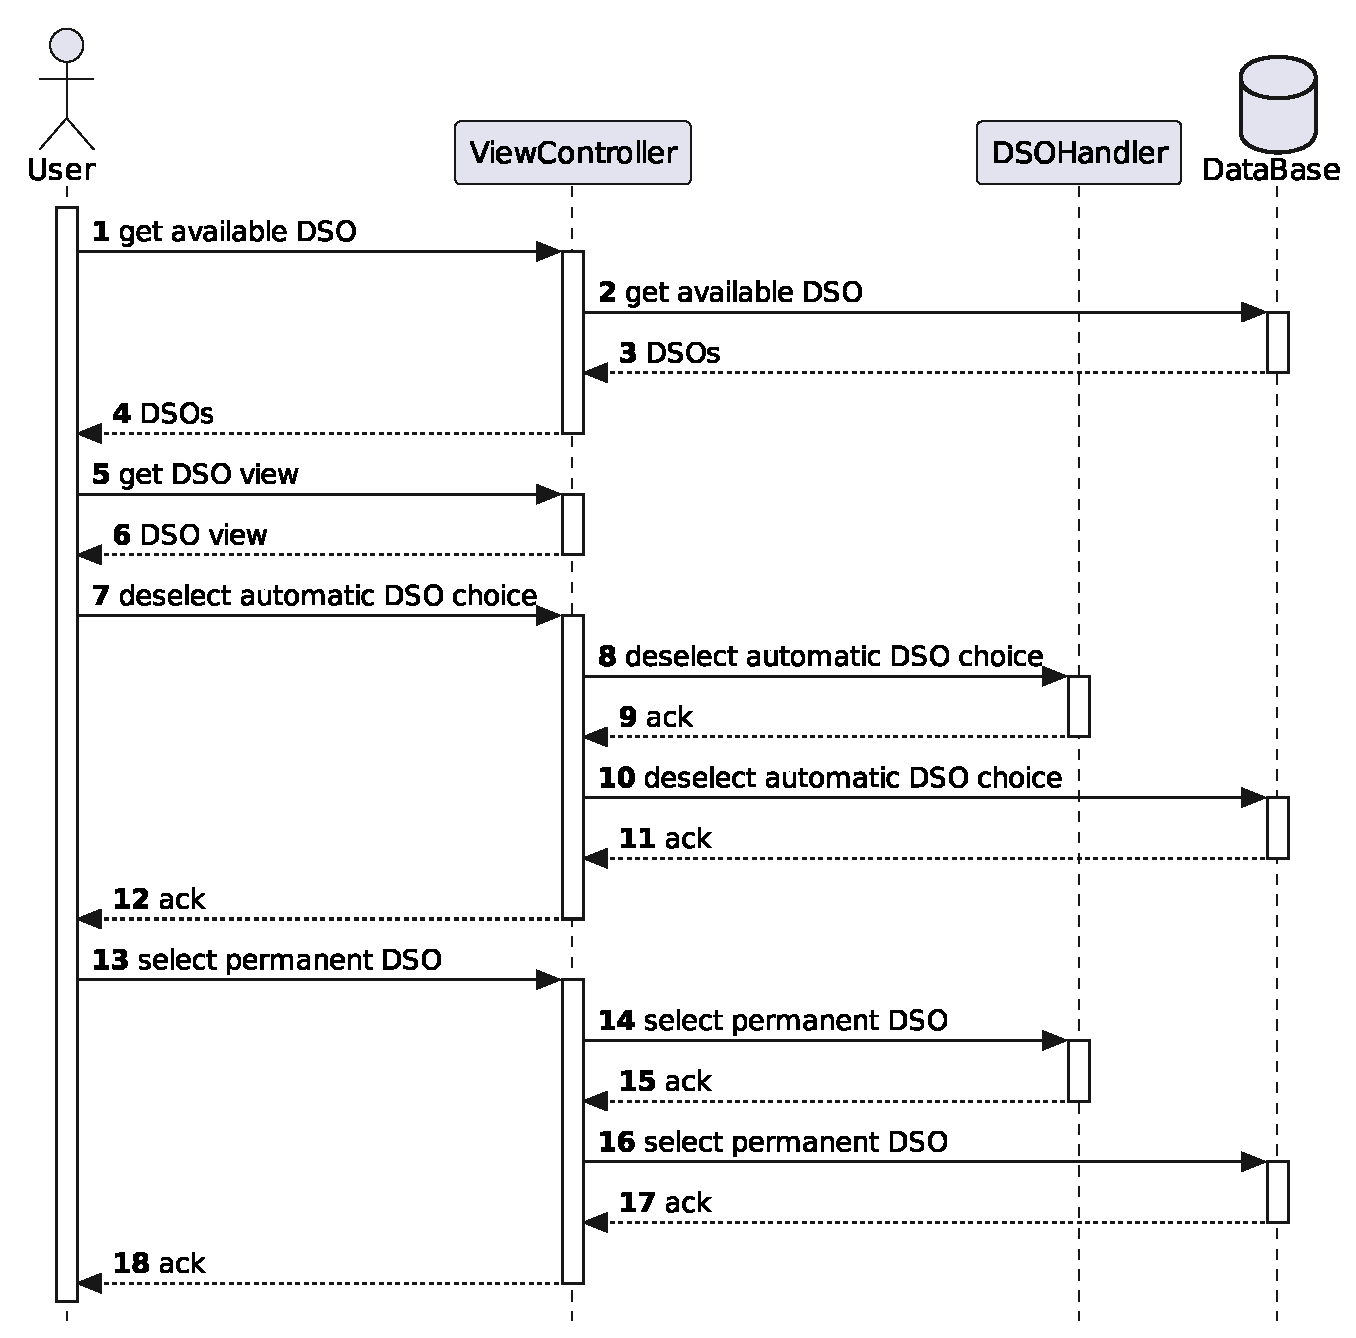
\includegraphics[width=0.85\columnwidth]{./images/diagrams/sequences/cpms/DSO}
    \caption{Caption}
\end{figure}

Instead of selecting a specific DSO, the user at the DSO view can also choose to activate/deactivate \doublequotes{Automatic DSO choice}, letting the system handle the DSO choice automatically or selecting the current DSO as permanent. In this view, it is also possible to modify the automatic payment method.

\pagebreak

\paragraph{CPMS | Create Special offer}

\begin{center}
    \begin{tabular}{ | >{\arraybackslash}m{0.17\columnwidth} | >{\arraybackslash}m{0.77\columnwidth} | }
        \hline
        \textbf{Identifier} & \showUC{uc:c:SpecialOffer} \\
        \hline
        \textbf{Actor} & CPO allowed user \\
        \hline
        \textbf{Entry condition} & The user is at the home page in the website \\
        \hline
        \textbf{Event flow} & \medskip\parbox[b][][b]{0.76\columnwidth}{
            \begin{enumerate}[nosep, leftmargin=*]
                \item The user selects \doublequotes{Special offers}
                \item The user selects \doublequotes{Create new special offer}
                \item The user inputs all the needed parameters
                \item The system creates a new special offer
            \end{enumerate}
        } \\
        \hline
        \textbf{Exit condition} & A new special offer is created \\
        \hline
        \textbf{Exceptions} & \medskip\parbox[b][][b]{0.76\columnwidth}{
            \begin{itemize}[nosep, leftmargin=*]
                \item Missing or wrong parameters
            \end{itemize}
        } \\
        \hline
    \end{tabular}
\end{center}

\begin{figure}[h!]
    \centering
    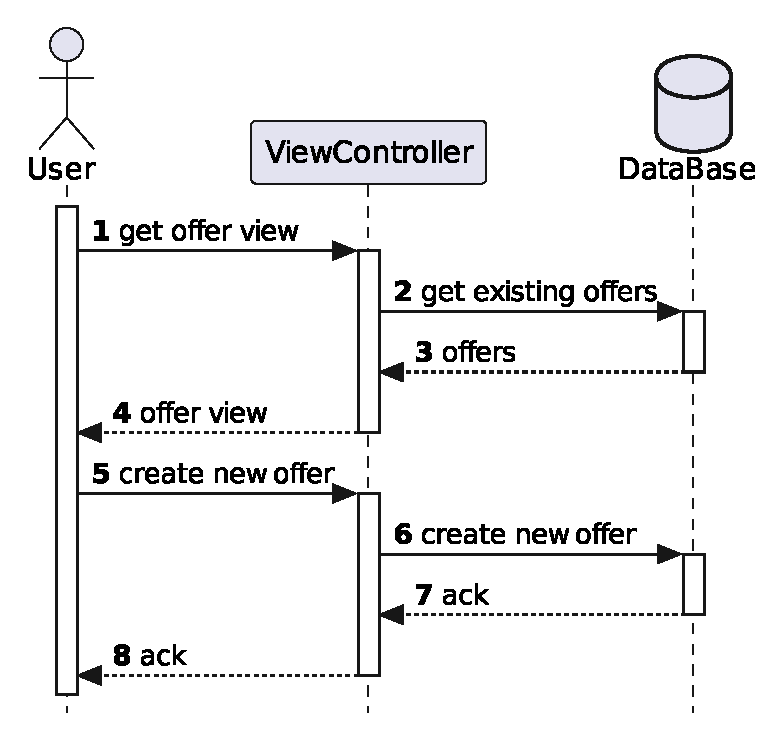
\includegraphics[width=0.45\columnwidth]{./images/diagrams/sequences/cpms/offers}
    \caption{a user creating a new special offer. In the special offer view users also see existing offers, and delete them if needed.}
\end{figure}

\pagebreak

\section{Performance requirements}

\paragraph{eMSP} The eMSP system should be generally responsive. It should provide answers to simple queries in less than 5 seconds, while more complex ones should complete in less than 30 seconds. If the system is directly interfacing with the user and the response isn't available after a couple of seconds, the frontend should display a loading indicator. A lower waiting time can be archived thanks to a proper database configuration and through the redundancy of components and data. The application performs much of the required computations on the backend, thus letting the application and the web interface only display the contents and doing some basic operations (sorting, checks\dots).

\paragraph{CPMS} Since the CPMS system is more geared towards monitoring, and eventually allows for some actions from the user, availability should be preferred over reliability. It's not essential that the system does not crush (although it is preferred), since all changes are immediately saved in permanent storage. It's more important that if the system crushes it can recover quickly, and all inputs are delivered as soon as possible and made permanent in the database storage. All the computation will take place on the servers of the system, which have to be replicated and distributed to better assert the desired availability and reach a consensus over the input received.

\section{Design constraints}

\subsection{Standards compliance}

Every system should correctly implement all the needed standard APIs for allowing interconnection with different pieces of software that expose those functionalities. Moreover, each system should be compliant with common payment APIs for managing user payments.

\subsection{Hardware limitations} \label{hwlimitations}

\paragraph{eMSP} For accessing the system, the user can use both the application which should be available in all the main mobile stores and should run on most of the devices present nowadays (e.g. an Android version greater or equal to 4.4 KitKat) or a browser which supports at least ES6 for correctly displaying all the views of the website.

\paragraph{CPMS} For accessing the system, any computer/laptop/tablet/phone with an installed web browser, connected to the internet, is sufficient, as a website is the sole user access point.

\section{Software system attributes}

\subsection{Reliability}

\paragraph{eMSP} The eMSP should be reliable, and even in case of failures, it should recover quickly. If downtimes, even if small, are frequent, this might make the user experience painful because of probably many failed requests.

\paragraph{CPMS} The CPMS website should be reliable enough to let users monitor and perform actions. Reliability is not to be preferred over availability. The CPMS servers on the other hand can be replicated to allow for higher reliability and protection of the data.

\subsection{Availability}

\paragraph{eMSP} The eMSP should be available 99\% of the time (about 361 days per year). Any longer unavailability period might encourage the user to move to some other competitor.

\paragraph{CPMS} The CPMS should be available 99.7\% of the time (about 364 days per year). Such a high availability is needed for the server to be responsive toward all end users, for better monitoring, and to secure that input actions are almost always registered.

\pagebreak

\subsection{Security}

\paragraph{eMSP} The eMSP should provide a high level of security for the information the users insert. Especially, the system must protect all the uploaded vehicles' information.

\paragraph{CPMS} The CPMS should provide a high level of security for the information the charging station dispatches. In particular, the system needs to be aware of \doublequotes{man in the middle} attacks where information coming from the stations is tampered with, which would result in incorrect automatic choices and eventually wrong information dispatched to the eMSP. Attention also should be paid to securing charging columns from possible manumissions in the validation of cars' certificates.

\subsection{Maintainability}

The system should follow basic design guidelines to make the whole system more maintainable. This will be described more deeply in the Design Document, but a general indication is to divide components into smaller ones, so that each one can do only a specific action, thus making the system easier to bring up and maintain, allowing also the maintenance of single components at a time.

\subsection{Portability}

\paragraph{eMSP} The backend should be able to run well on Linux systems, and it should be optimized to use all the standard Linux and POSIX features. The website should instead work well on all the major browsers, while the mobile application should be able to run on many architectures, allowing it to work on all the supported devices, as described in \reference{hwlimitations}.

\paragraph{CPMS} The backend should be able to run well on Linux systems, and it should be optimized to use all the standard Linux and POSIX features. The database system should be distributed for higher availability.
